\documentclass[]{beamer}
\usetheme{KUL}
\usepackage{multirow}
\usepackage{multicol}
\usepackage{tikz}
\usepackage{ulem}
\usepackage{siunitx}
\newcommand\itemS{\item[\textbf{\S}]}
\definecolor{darkgreen}{rgb}{0,0.598,0.199}
\usepackage{times} % set font on times new roman
\usepackage{eurosym} % package for Euro sign
\usepackage{lineno}   % package for line numbering
\usepackage{hyperref} % this is for url links
\usepackage{subcaption}  % this package enables one to put several figures next to each other
%\usepackage{capt-of}
\usepackage{textcomp}
\usepackage{setspace}
\usepackage{gensymb}
%\usepackage[font=small]{caption}
\usepackage{diagbox}
\usepackage[ruled,vlined,spanish,onelanguage]{algorithm2e}
\newenvironment{figure*}%
{\begin{figure}}
{\end{figure}}
\captionsetup[figure]{labelformat=empty, font=scriptsize}
\captionsetup[table]{labelformat=empty, font=scriptsize}
%\captionsetup{font=scriptsize, labelfont=scriptsize}
%----------------------------------
% Fill in the essential Information
%----------------------------------

\title[Individualizaci\'on de filamentos mediante optimizaci\'on]{Defensa de Tesis: Individualizaci\'on de filamentos en una red mediante optimizaci\'on}
%\subtitle{\ldots a subtitle}
\author[L.\ Pizarro]{Leonardo Pizarro} % between [] is short name, between {} is long name
\date{\today} % Here you can also just type something, e.g. October 10, 2017
%\institute[DCC - FCFM - UChile]{Magister en Ciencias de la Computaci\'on\\Facultad de Ciencias F\'isicas y Matem\'aticas\\ Departamento de Ciencias de la Computaci\'on \\ Universidad de Chile}
\institute[]{Profesor Gu\'ia: Mauricio Cerda\\Profesor Co-gu\'ia: Jacques Dumais}

%----------------------------------
% ACTUAL PRESENTATION STARTS HERE
%----------------------------------

\begin{document}

% TITLE PAGE	
	{
		\setbeamertemplate{headline}{} %define local, empty header for title page
		\setbeamertemplate{footline}{} %define local, empty footer for title page
		\maketitle
	}
	\addtocounter{framenumber}{-1} % We don't count the title page

\begin{frame}
\frametitle{Contenidos} 
\tableofcontents
\end{frame}

\section{Motivaci\'on y Antecedentes}
% [allowframebreaks] para dividir en multiples frames
\begin{frame}{¿Qu\'e es un filamento?}
    \begin{columns}
    \begin{column}{0.32\textwidth}
        \begin{itemize}
            \item Estructuras alargadas con diferentes propiedades
            \item Observaci\'on de Microscop\'ia
            \begin{itemize}
            \small
                \item Ruido
                \item Resoluci\'on
            \end{itemize}
        \end{itemize}
    \end{column}
    \begin{column}{0.68\textwidth}
        \begin{figure*}[h]
          \centering
            \begin{subfigure}[t]{0.48\textwidth}
            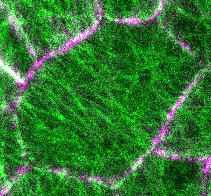
\includegraphics[height=1.2in]{Pictures/small_MT.jpg}
            \end{subfigure}
            ~ 
            \begin{subfigure}[t]{0.48\textwidth}
            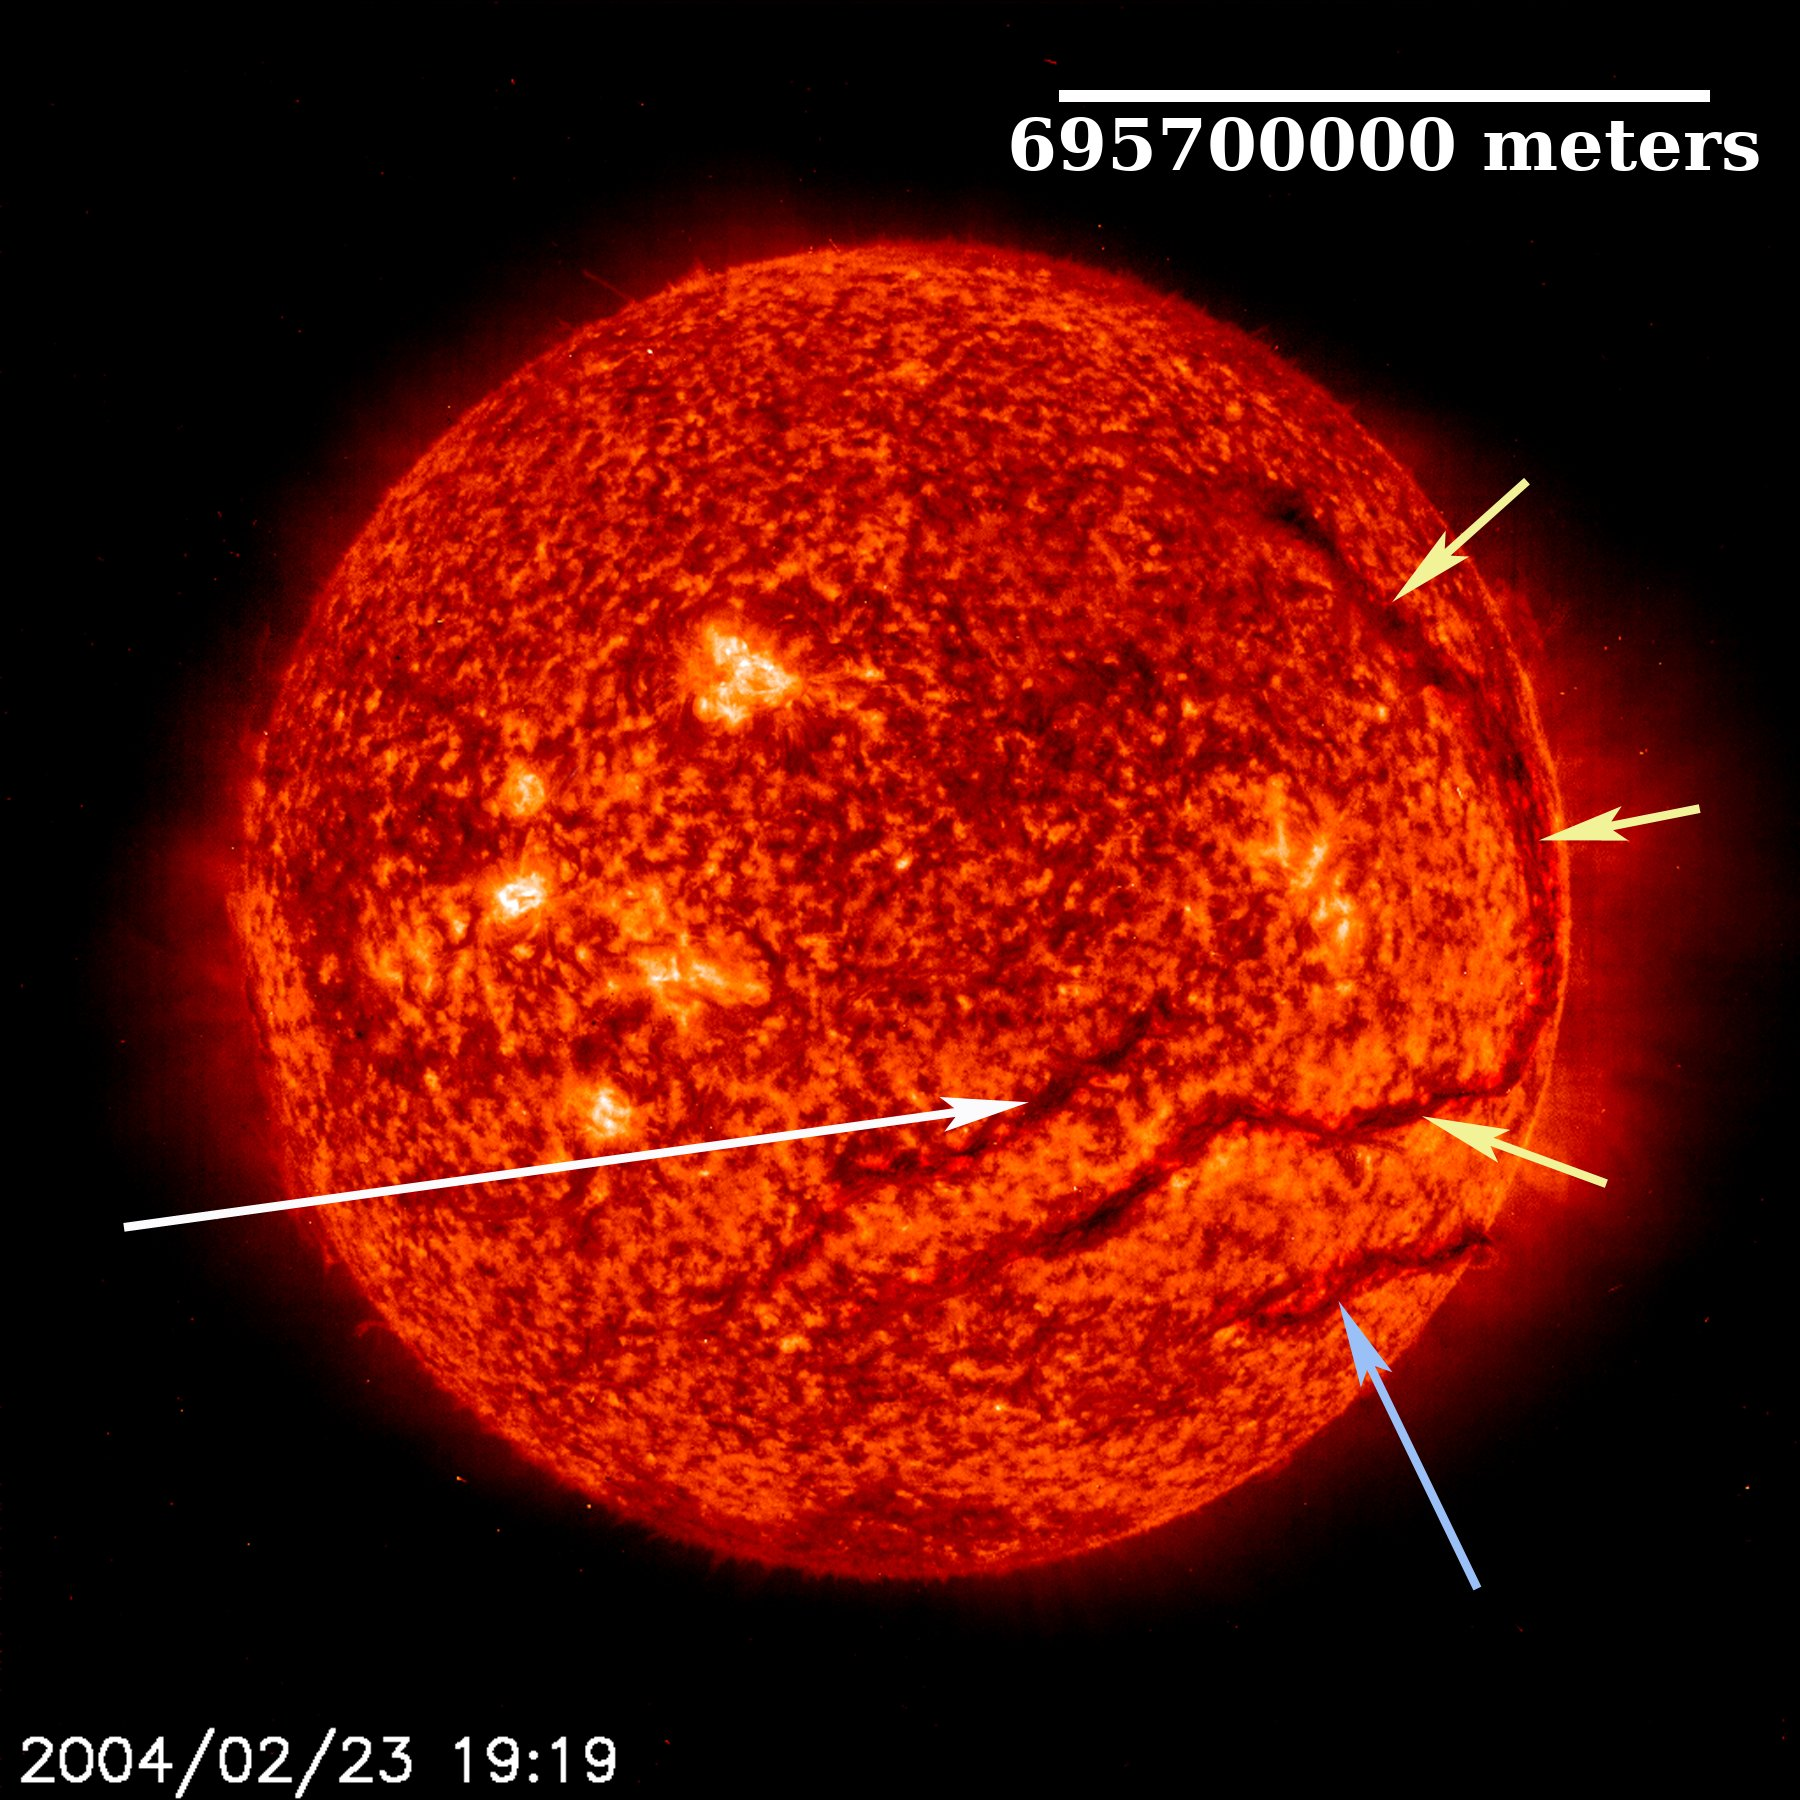
\includegraphics[height=1.2in]{Pictures/sun_filament.jpg}
            \end{subfigure}
            \vspace{0.5cm}
             \begin{subfigure}[t]{\textwidth}
             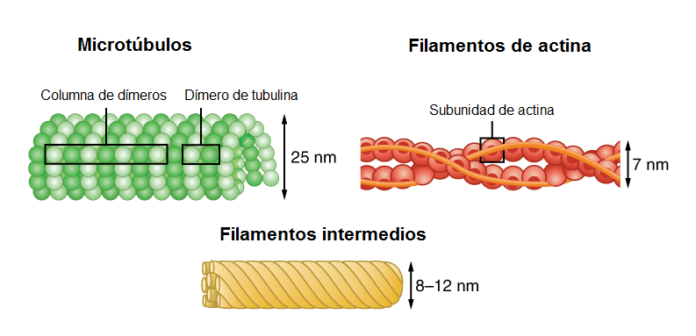
\includegraphics[height=1.2in]{Pictures/citoesqueletoo-min.png}
            \end{subfigure}
    
        \end{figure*}
    \end{column}
\end{columns}
\end{frame}

\begin{frame}{Varias soluciones posibles}
  \begin{columns}
    \begin{column}{0.6\textwidth}
    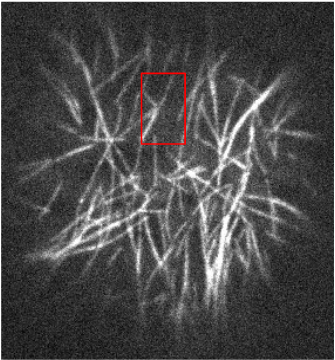
\includegraphics[scale=0.5]{Pictures/NoConsenso.png}
    \end{column}
    \begin{column}{0.2\textwidth}
    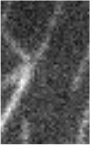
\includegraphics[scale=0.5]{Pictures/NoConsenso2.png}
    \end{column}
    \begin{column}{0.2\textwidth}
    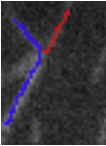
\includegraphics[scale=0.5]{Pictures/NoConsenso3.png}
    \vspace{0.5cm}
    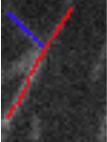
\includegraphics[scale=0.5]{Pictures/NoConsenso4.png}
    \end{column}
\end{columns}
\end{frame}

\begin{frame}{Dificultades del Problema}
    \begin{itemize}
        %\item Variaci\'on de las caracter\'isticas de filamentos entre diferentes c\'elulcas
        \item Desconocimiento de los puntos de inicio y fin de un filamento
        \item Necesidad de incorporar m\'as descriptores de los filamentos
        \item Resoluci\'on y Ruido en las im\'agenes
        \item Diferencias en el comportamiento de los filamentos dependiendo de la c\'elula observada.
    \end{itemize}
\end{frame}

\begin{frame}{Familias de M\'etodos}
    \hspace{-1cm}
    \centering
    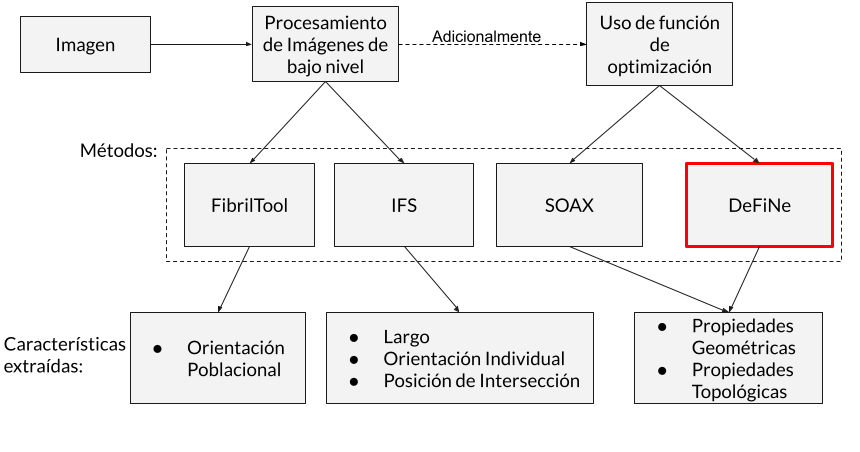
\includegraphics[height=2.4in]{Pictures/familiasDeMetodos.png}
\end{frame}

%\subsection{M\'etodos basados en Vision por Computador}
\begin{frame}{Extracci\'on de redes de MT}
    
    \begin{columns}
    \hspace{-1cm}
        \begin{column}{0.25\textwidth}
            \centering
            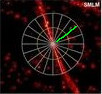
\includegraphics[height=1.4in]{Pictures/MT-LFT.jpeg}
        \end{column}
        \begin{column}{0.75\textwidth}
            \centering
            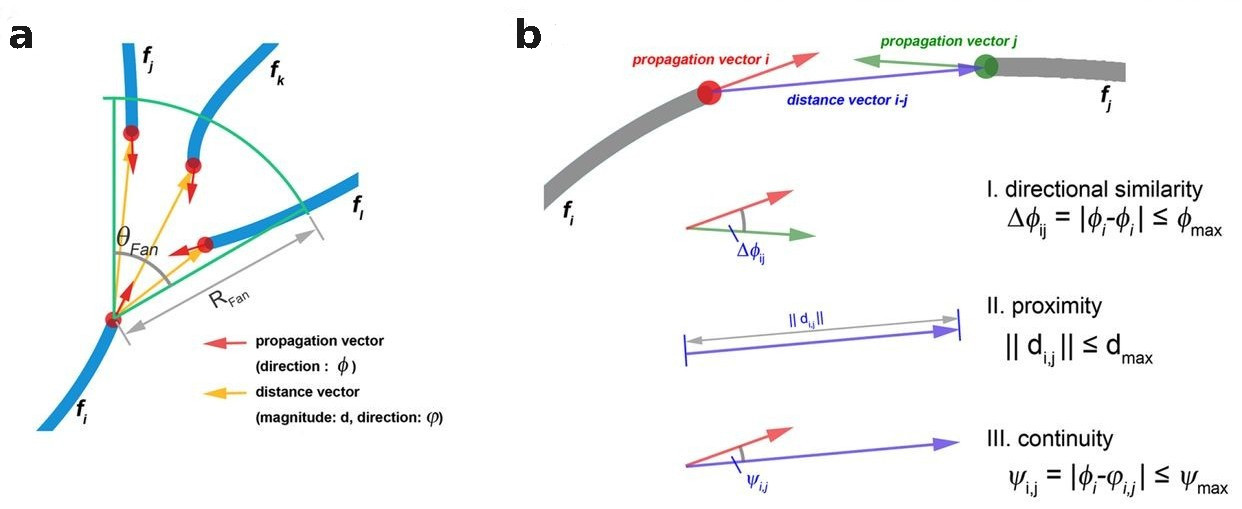
\includegraphics[height=1.4in]{Pictures/MT-OFT.jpeg}
        \end{column}
    \end{columns}
    %\vspace{1cm}
    \begin{figure}
        %\includegraphics{}
        \caption{Zhen Zhang, Yukako Nishimura, and Pakorn Kanchanawong. Extracting microtubule networks from superresolution single-molecule localization microscopy data. Molecular biology of the cell, 28(2):333–345, 2017.}
    \end{figure}
    % \begin{itemize}\fontsize{8pt}{7.2}\selectfont
    %     \item 
    % \end{itemize}
\end{frame}

\begin{frame}{Quantitative IFS}
    \begin{figure}[h]
        \centering
        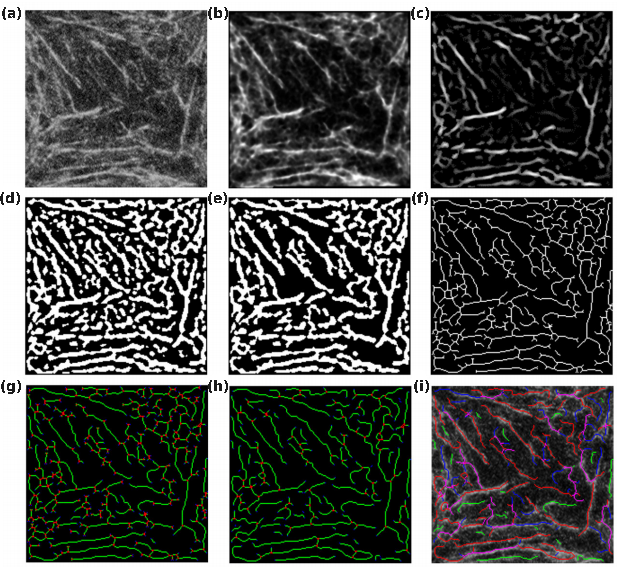
\includegraphics[height=2.3in]{Pictures/QuantitativeIFS.png}
        \caption{Jun Qiu and F LI. Quantitative morphological analysis of curvilinear network for microscopic image based on individual fibre segmentation (ifs). Journal of microscopy, 256(3):153–165, 2014}
    \end{figure}
\end{frame}

%\subsection{M\'etodos basados en Optimizaci\'on}
\begin{frame}{SOAX}
    \begin{figure}
        \centering
        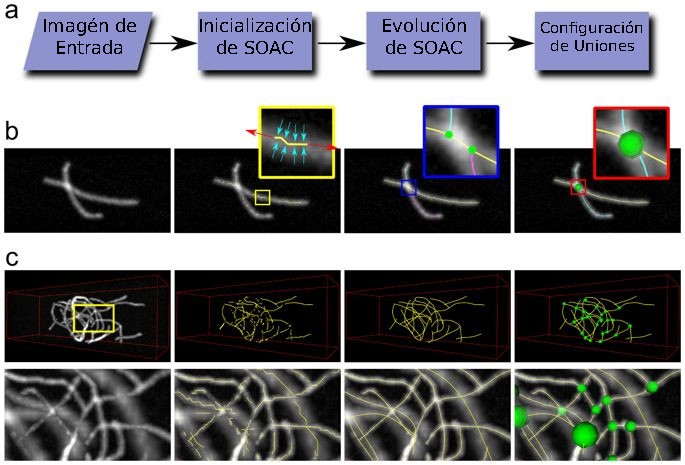
\includegraphics[height=2.1in]{Pictures/SOAX_translated.jpg}
        \caption{Ting Xu, Dimitrios Vavylonis, Feng-Ching Tsai, Gijsje H Koenderink, Wei Nie, Eddy Yusuf, I-Ju Lee, Jian-Qiu Wu, and Xiaolei Huang. Soax: a software for quantification of 3d biopolymer networks. Scientific reports, 5:9081, 2015.}
    \end{figure}
\end{frame}

\begin{frame}{DeFiNe}
    %\vspace{-1cm}
    \begin{columns}
        \begin{column}{0.55\textwidth}
            \begin{itemize}\fontsize{9pt}{5}\selectfont
                \item Conjunto de aristas $\rightarrow$ camino/filamentos
                \item Recorrer los P caminos es NP-Hard
                \item Similitud con un {\it Path Cover Problem} $\rightarrow$ FCP
            \end{itemize}        
        \end{column}
        \begin{column}{0.45\textwidth}
            \begin{itemize}\fontsize{9pt}{7.2}\selectfont
                \item 2 Heur\'isticas para crear {\bf P'}
                \item {\bf P'} $\rightarrow$ {\it Set Cover Problem}
                \item {\it SCP} usa 1 propiedad para ponderar aristas
            \end{itemize}
        \end{column}
    \end{columns}
    \begin{figure}
        \centering
        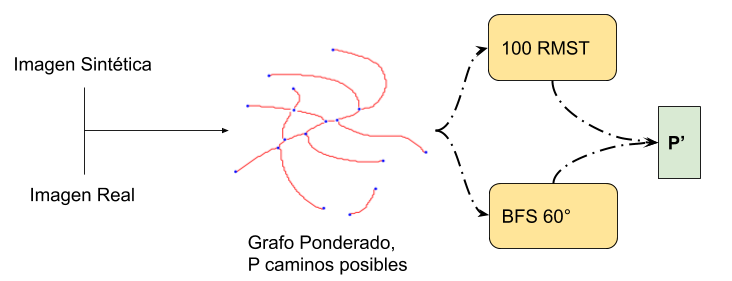
\includegraphics[scale=0.42]{Pictures/flujoDefine2.png}
        \caption{David Breuer and Zoran Nikoloski. Define: an optimisation-based method for robust disentangling of filamentous networks. Scientific reports, 5:18267, 2015.}
    \end{figure}
\end{frame}


\begin{frame}{M\'etodos basados en:}
    \begin{columns}
        \begin{column}{0.4\textwidth}
             \begin{itemize}
                \item Vision por Computador
                \item Optimizaci\'on
                \begin{itemize}
                    \item Metaheur\'istica ACO
                \end{itemize}
            \end{itemize}
        \end{column}
        \begin{column}{0.6\textwidth}
            \begin{itemize}
                \item Muchos par\'ametros
                \item Diferencia entre m\'etodos: Una Soluci\'on vs b\'usqueda de la mejor soluci\'on
                \item Problema gen\'erico: Obtener par\'ametros de los expertos (sesgo)
            \end{itemize}
        \end{column}
    \end{columns}
\end{frame}

\begin{frame}{Individualizaci\'on de Filamentos como un Problema de Satisfacci\'on de Restricciones}
    \begin{itemize}
    \item Se desconoce a priori el n\'umero de filamentos a buscar.%, dado que una imagen puede tener individualizaciones distintas para 2 expertos.
    \item Generalmente se busca individualizar m\'as de un filamento por imagen, lo que conlleva a elegir los mejores filamentos entre las soluciones que se encuentren.
    \item El uso de un grafo para representar la red de filamentos puede implicar que las combinaciones de soluciones crezcan de manera exponencial.
\end{itemize}
\end{frame}

\section{Hip\'otesis y Objetivos}
\begin{frame}{Hip\'otesis}
\small
    \begin{itemize}
        \item A partir de un grafo con pesos, no dirigido, con o sin ciclos, que representa una red de filamentos, en conjunto con utilizar una combinaci\'on de caracter\'isticas de los segmentos de filamentos como largo, grosor, \'angulo de bifurcaci\'on o curvatura, sumado a la incorporaci\'on de informaci\'on previa disponible sobre el tipo de c\'elula (red de filamentos con o sin ciclos), es posible identificar a cada filamento en la red resolviendo un modelo de optimizaci\'on.
    \end{itemize}
\end{frame}

\begin{frame}{Objetivo General}
\small
    \begin{itemize}
        \item Desarrollar un modelo de optimizaci\'on para la individualizaci\'on de filamentos a partir de un grafo representativo de la red de filamentos, evaluando la variaci\'on en el resultado con distintas combinaciones entre las propiedades de cada segmento de filamento como el grosor, largo, \'angulo de bifurcaci\'on o direcci\'on.
    \end{itemize}
\end{frame}


\begin{frame}{Objetivos Espec\'ificos}
\small
\begin{enumerate}
    \item[OE 1] Generar un modelo de optimizaci\'on %para la identificaci\'on de filamentos a partir de un grafo con pesos que representa la red de filamentos.
    \item[OE 2] Implementar un algoritmo que resuelva el modelo de optimizaci\'on %, entregando como salida la identificaci\'on de filamentos, considerando casos de solapamiento y/o cruce.
    \item[OE 3] Identificar la ponderaci\'on de propiedades en casos espec\'ificos: microt\'ubulo y neurona %que entregue mejores resultados % para grafos que representen una neurona, una bacteria y una c\'elula eucariota de planta.
    \item[OE 4] Evaluar y comparar t\'ecnicas del estado del arte% que usan s\'olo herramientas de visi\'on por computador, basada en poblaci\'on de p\'ixeles, o que utilizan un m\'etodo derivado de contornos activos.
    %una soluci\'on exacta o aproximada respecto a la individualizaci\'on, dependiendo de la complejidad computacional del problema. 
\end{enumerate}
    
\end{frame}

\section{Hormigas}
%\subsection{Metaheur\'istica ACO }
\begin{frame}{Hormigas (OE 1)}
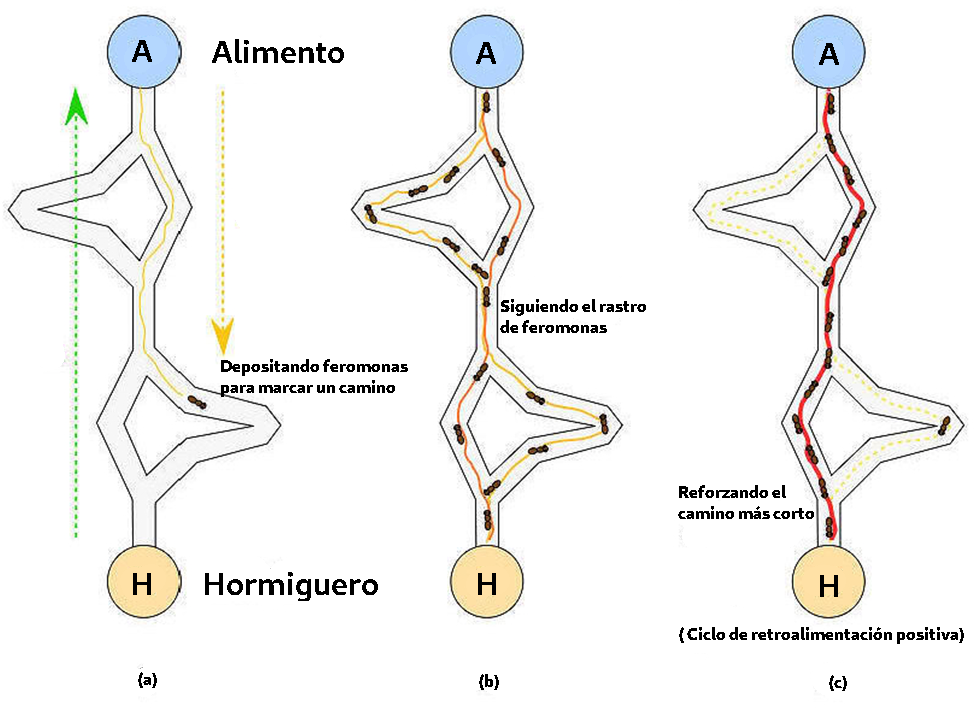
\includegraphics[width=0.95\textwidth]{Pictures/ACO-ant.png}
\end{frame}

\begin{frame}{Hormigas (OE 1)}
\centering
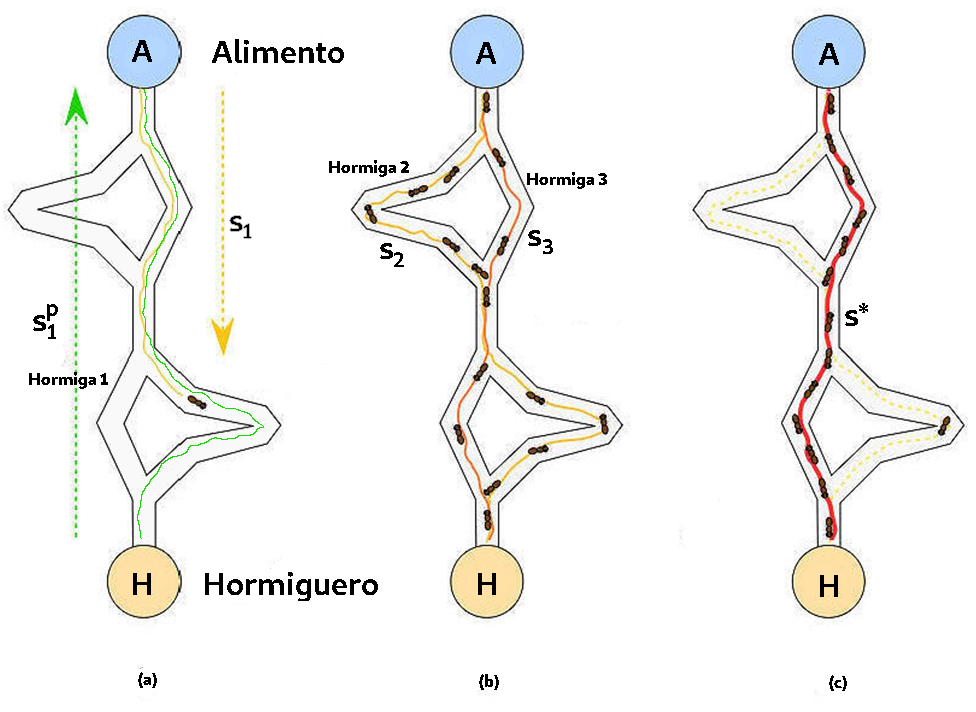
\includegraphics[width=0.95\textwidth]{Pictures/ACO-ant-2.png}
\end{frame}

\begin{frame}{Modelo de Feromonas (OE 1)}
\small
\begin{itemize}
    \item Comunicaci\'on indirecta mediante feromonas
    \item Recorrido aleatorio
    \item Convergencia sobre el camino m\'as corto
    \item Opciones de caminos posibles representan el espacio de b\'usqueda
    \item Orden no estricto
\end{itemize}
    \begin{algorithm}[H]
    \SetAlgoLined
     Ajuste de Par\'ametros \& inicializaci\'on de feromonas\;
     \While{Criterio de finalizaci\'on no se cumple}{
       Construcci\'on\_de\_soluci\'on\_de\_cada\_hormiga()\;
       M\'etodo\_de\_b\'usqueda\_no\_local(); //Paso opcional\\
       Actualizaci\'on\_de\_feromonas()\;
     }
     \caption{Algoritmo metaheur\'istica ACO}\label{ACO-Algo}
    \end{algorithm}
\end{frame}

\begin{frame}{Adaptaci\'on de ACO a un problema de satisfacci\'on de restricciones (OE 1)}
    \begin{itemize}
        \item Hormigas Sint\'eticas o Agentes
        %\item Basado en el comportamiento de las hormigas reales
        \item Entendiendo los caminos posibles a recorrer por las hormigas como un grafo
        \item Camino $s$ compuesto por aristas o componentes de soluci\'on $c_i$
        \item Valor de la feromona depositada $\tau_{i}$
        \item Se pueden agregar restricciones $\Omega$ en el desplazamiento
    \end{itemize}
\end{frame}

%\subsection{Problema de Satisfacci\'on de Restricciones}
\begin{frame}{ACO aplicado como Problema de Satisfacci\'on de Restricciones (OE 1)}
  \begin{columns}
    \begin{column}{0.5\textwidth}
        \begin{itemize}
          \item $P = (S, \Omega, F)$
          % esta definido por un conjunto discreto de variables
          \item S:  Cjto. de soluciones, compuesto por variables discretas $X_{i}$, $i \in 1 \dotsc n$
          %\item $S:\quad X = v_{i}^{j} \in D_{i} = \{v_{i}^{1} \dotsc  v_{i}^{|D_{i}|}\}$.
          \item Sol. Candidata $s \in S$, y $s^{*}$ una soluci\'on \'optima
          \item Cjto. de Restricciones $\Omega$
          \item Funci\'on objetivo $F: S\rightarrow \mathbb R_{0}^{+}$
          %\item  
          
      \end{itemize}
    \end{column}
    \begin{column}{0.5\textwidth}
      \begin{itemize}
          \item $s$ es factible si satisface las restricciones de $\Omega$
          % y se relacionan mediante 
          \item Pueden existir m\'ultiples soluciones $s^{*}$
          \item $S^{*}$ es el conjunto que engloba todas las soluciones \'optimas
          \item $s^{*} \in S^{*} \subseteq S$
      \end{itemize}
    \end{column}
\end{columns}
\end{frame}





% \begin{frame}{Adaptaci\'on a Individualizaci\'on de Filamentos}
%     \begin{algorithm}[H]
%     \SetAlgoLined
%     \KwData{Variables $X_i \dotsc X_n$, dominios $D_1 \dotsc D_n$, Restricciones $\in \Omega$}
%     \KwResult{conjunto s\textquotesingle $ \subseteq S$ != $\emptyset$, si existen soluciones factibles}
%      Ajuste de Par\'ametros \& inicializaci\'on de feromonas \;
%      \While{Criterio de finalización no se cumple}{
%       Construcci\'on\_de\_soluci\'on\_de\_cada\_hormiga()\;
%       M\'etodo\_de\_b\'usqueda\_no\_local(); //Paso opcional\\
%       Actualizaci\'on\_de\_feromonas()\;
%      }
%      \caption{Algoritmo de un modelo COP adaptado a una metaheur\'istica ACO}\label{COP-ACO-Algo}
%     \end{algorithm}
% \end{frame}


\section{Algoritmo Propuesto}
%\subsection{Inicializaci\'on de Par\'ametros}
\begin{frame}{Inicializaci\'on de Par\'ametros en ACO (OE 1)}
    \begin{columns}
        \hspace{-1cm}
        \begin{column}{0.45\textwidth}
            \begin{itemize} \fontsize{9pt}{5}\selectfont
                \item Umbral $\theta$: 
                \begin{itemize} \fontsize{9pt}{5}\selectfont
                    \item $[0, \theta]$
                    \item $]\theta, Max\_Angle]$
                \end{itemize}
                \item Umbral $Max\_Angle$: 
                \begin{itemize} \fontsize{9pt}{5}\selectfont
                    \item $max(2.5 \theta, 90\degree)$
                    \item $\measuredangle (e_{i}, e_{j})> Max\_Angle$
                \end{itemize}
                \item Factor {\it Max\_Axial\_Displacement}: Curvatura y Magnitud entre segmentos
                \item {\it Max\_Score}
                \item Valor Inicial $\tau_0$
                \item Criterio de finalizaci\'on de un recorrido
            \end{itemize}
        \end{column}
        \begin{column}{0.55\textwidth}
        %\vspace{-2cm}
            \centering
            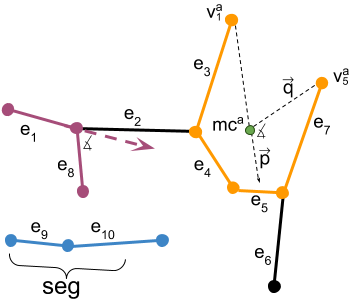
\includegraphics[scale=0.55]{Pictures/ant-params.png}
        \end{column}
    \end{columns}
\end{frame}

%\subsection{Construcci\'on de Soluciones}
\begin{frame}{ACO: Construcci\'on de Soluci\'on (OE 1)}
\centering
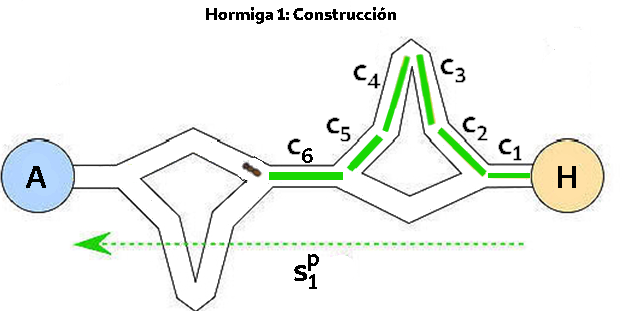
\includegraphics[scale=0.4]{Pictures/ACO-ant-Constr.png}
\begin{itemize}
    \item Influencia de feromonas $\tau$ y de una heur\'istica $\eta$ en la elecci\'on de Aristas/Componentes $c_i$ que respeten restricciones en $\Omega$
    \item Aspecto aleatorio en la elecci\'on
\end{itemize}
\end{frame}

% \begin{frame}{ACO: Heur\'istica de Asignaci\'on Inicial}
% \begin{enumerate}
% \item Arista $a: (n_i,n_j)$ tal que $deg(n_i) = 1$ o $deg(n_j) = 1$ 
% %La arista a asignar debe tener al menos uno de sus nodos con grado 1, indicando que es el inicio o final de una parte del grafo.

% \item De no haber aristas disponibles con esas caracter\'isticas, se realiza una asignaci\'on inicial de una arista que cumpla con 2 criterios:
% \begin{itemize}
%     \item $a: (n_i,n_j)$ tal que $deg(n_i) >= 2$ o $deg(n_j) >= 2$ 
%     \item El \'angulo que forma la arista candidata a elegir, junto a otra arista a la que pertenece el nodo, debe pertenecer al rango $]\theta, Max\_Angle]$.
% \end{itemize}

% \item Una arista aleatoria que no pertenezca a una soluci\'on o camino evaluado como de buena calidad
% %. La calidad de un camino se presenta m\'as adelante en esta secci\'on.
% \end{enumerate}
% \end{frame}

\begin{frame}{ACO: Construcci\'on de Soluci\'on, 1ra Arista (OE 1)}
    \centering
    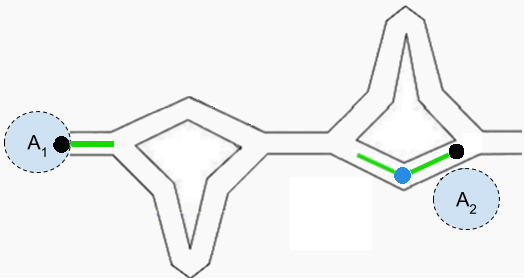
\includegraphics[scale=0.5]{Pictures/ant-initial-edge.png}
    \begin{itemize}
        \item Heur\'istica de Asignaci\'on Inicial: 3 criterios
        \item Enfoque en la exploraci\'on del espacio de b\'usqueda
    \end{itemize}
\end{frame}

\begin{frame}{ACO: Construcci\'on de Soluci\'on (OE 1)}
\centering
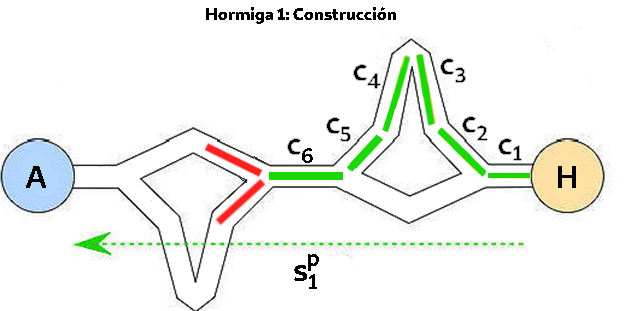
\includegraphics[scale=0.35]{Pictures/ACO-ant-Constr-choices.png}
        \begin{equation}
P(c_{i} | s^{P}) = \frac
        {\tau_{i}^{\alpha} ~ \eta_{i}^{\beta}}
        {\sum\limits_{c_{i}\in N(s^p)}{\tau_{i}^{\alpha} ~ \eta_{i}^{\beta} } }, \forall c_{i} \in N(s^{P}).
\label{eq:antProbabilities}
\end{equation}
\end{frame}

\begin{frame}{ACO: Construcci\'on de Soluci\'on (OE 1)}
\centering
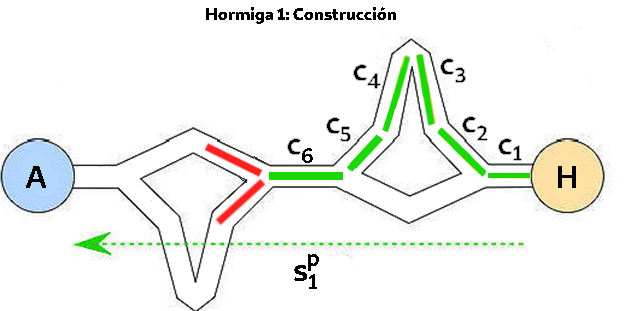
\includegraphics[scale=0.4]{Pictures/ACO-ant-Constr-choices.png}
\begin{itemize}
    \item Calidad $s^{P}_1$ = $\sum \eta_{i}$
    \item Calidad $s_1$ = $\frac{1}{n}\sum \eta_{i} $
    \item Calidad M\'inima $\geq \frac{Max\_Score}{2}$
    \item Buena Calidad: $Max\_Score$
    \item Calidad Intermedia: $[\frac{Max\_Score}{2}, Max\_Score[$
\end{itemize}
\end{frame}

%\subsection{M\'etodo de b\'usqueda no local}
\begin{frame}{B\'usqueda no local: l\'ogicas globales/centralizadas (OE 1)}
    
    \begin{columns}
        \begin{column}{0.4\textwidth}
            \begin{itemize}
                \item Eliminar soluciones candidatas que no aporten informaci\'on nueva
                \item Soluciones parcialmente repetidas
            \end{itemize}
        \end{column}
        \begin{column}{0.2\textwidth}
        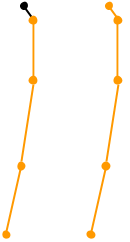
\includegraphics[scale=0.5]{Pictures/ant-segments-repetead-sol1.png}
        \end{column}
        \begin{column}{0.2\textwidth}
        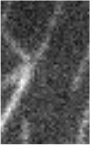
\includegraphics[scale=0.5]{Pictures/NoConsenso2.png}
        \end{column}
        \begin{column}{0.2\textwidth}
        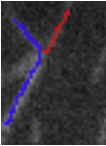
\includegraphics[scale=0.5]{Pictures/NoConsenso3.png}
        \vspace{0.5cm}
        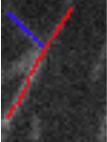
\includegraphics[scale=0.5]{Pictures/NoConsenso4.png}
        \end{column}
    \end{columns}
\end{frame}

\begin{frame}{ACO: Actualizaci\'on de Feromonas (OE 1)}
\centering
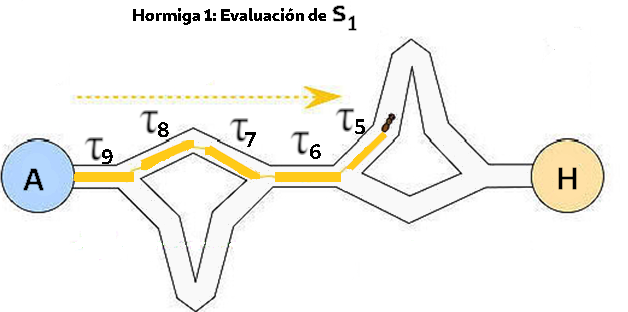
\includegraphics[scale=0.4]{Pictures/ACO-ant-ferom.png}
\begin{itemize}
    \item Evaluaci\'on de factiblidad de soluciones candidatas $s \in S$
    \item Premiar los caminos de buena calidad
    \item Prop\'osito: Convergencia sobre un camino \'optimo
\end{itemize}
\end{frame}


%\subsection{Anti-feromonas}
\begin{frame}{Anti-feromonas SAP (OE 1)}
\centering
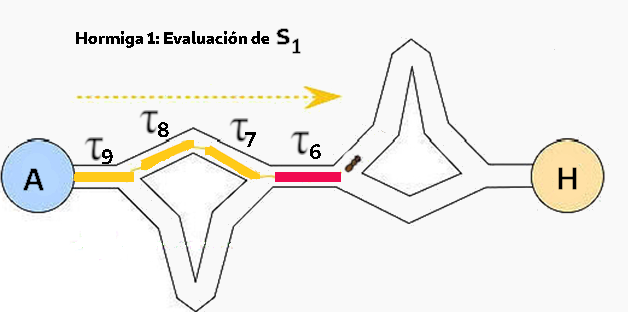
\includegraphics[scale=0.4]{Pictures/ACO-ant-ferom-penalize.png}
    \begin{itemize}
        \item Cambio: $\tau_0 \longrightarrow \gamma$
        \item $\gamma$ es un factor penaliza los caminos de mala calidad
        \item 2 penalizaciones $\longrightarrow \tau_i = 0$ 
    \end{itemize}
\end{frame}

\begin{frame}{Problema de Anti-feromonas SAP (OE 1)}
\centering
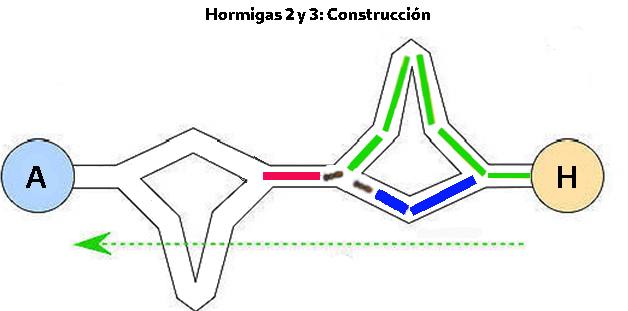
\includegraphics[scale=0.4]{Pictures/ACO-ant-constr-penalize.png}
    \begin{itemize}
        \item Problema: penalizaci\'on puede ocasionar perdida de soluciones factibles
        \item Propuesta: Relacionar penalizaci\'on de $\tau_i$ con $c_i \in s^P$
    \end{itemize}
\end{frame}

\begin{frame}{Anti-feromonas SAP dependientes del camino previo (OE 1)}
    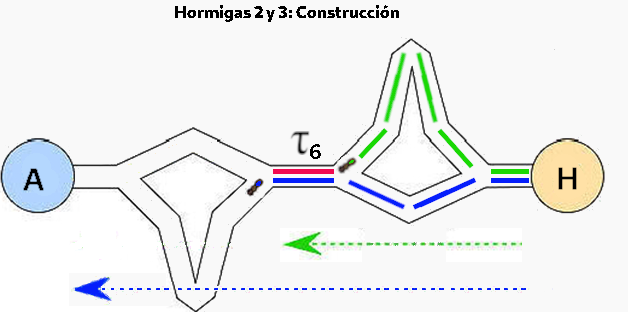
\includegraphics[scale=0.51]{Pictures/ACO-ant-ferom-penalize-seg.png}
\end{frame}


\begin{frame}{Extensi\'on de Anti-feromonas sobre un segmento (OE 1)}
\centering
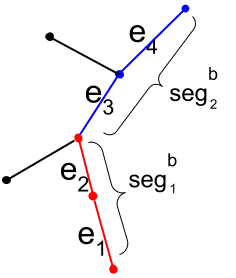
\includegraphics[scale=0.4]{Pictures/ant_segments_simple_case.png}
    \begin{itemize}
        \item Cada arista del segmento forma un \'angulo en el rango $[0, \theta]$ con sus vecinos
        \item Penalizaci\'on de $e_3$ se asocia al $seg^{b}_{1}$, sin perjudicar otros caminos que pasen por $e_3$ pero no por el segmento $seg^{b}_{1}$.
    \end{itemize}
\end{frame}

\begin{frame}{Anti-feromonas sobre un segmento de una sola arista (OE 1)}
\centering
\begin{figure*}
  \begin{subfigure}[t]{0.48\textwidth}
    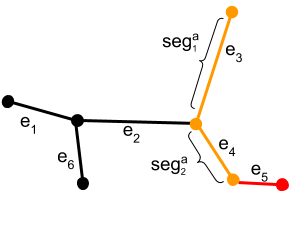
\includegraphics[scale=0.5]{Pictures/ant_segments_complex_case_B2.png}
  \end{subfigure}%
    ~ \hspace{0.1cm}
    \begin{subfigure}[t]{0.48\textwidth}
    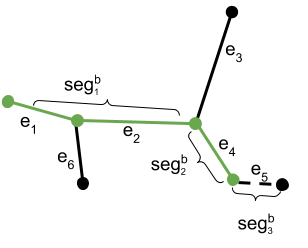
\includegraphics[scale=0.5]{Pictures/ant_segments_complex_case_B_blocked.png}
    \end{subfigure}
\end{figure*}
\begin{itemize}
    \item Segmentos de una sola arista ocasionan mismo problema que se intenta resolver
\end{itemize}
\end{frame}

\begin{frame}{Anti-feromonas sobre un segmento (OE 1)}
\centering
    
\includegraphics[scale=0.5]{Pictures/ant_segments_complex_case_B2_extended.png}
    \begin{itemize}
        \item Se extiende el segmento unitario con el segmento que lo precede
    \end{itemize}
\end{frame}

%\subsection{Criterios para la Actualizaci\'on de Anti-feromonas}
\begin{frame}{Anti-feromonas sobre soluciones de calidad intermedia (OE 1)}
\begin{itemize}
    \item Curvatura de una soluci\'on
    \item Magnitud de desplazamiento entre segmentos
    \item Criterio espec\'ifico para neuronas
\end{itemize}
\end{frame}

\begin{frame}{Curvatura de una soluci\'on (OE 1)}
\centering
    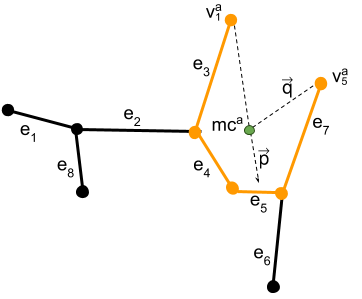
\includegraphics[scale=0.5]{Pictures/ant_curvature_case.png}
    \begin{itemize}
        \item El \'angulo entre la proyecci\'on de $\Vec{p}$ y $\Vec{q}$ debe ser menor a $\theta \times Max\_Axial\_Displacement$ para no descartar la soluci\'on.
    \end{itemize}
\end{frame}

\begin{frame}{Magnitud de desplazamiento entre segmentos (OE 1)}
    \begin{figure*}[h]
    \centering
    \begin{subfigure}[t]{0.45\textwidth}
        \centering
        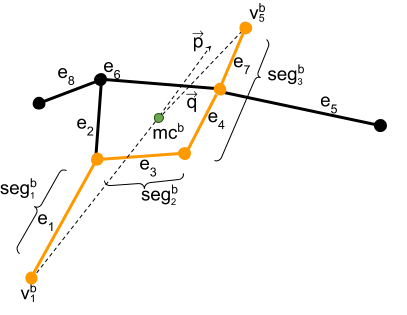
\includegraphics[scale=0.4]{Pictures/ant_segmentMagnitude_case.png}
    \end{subfigure}
    ~ \hspace{0.5cm}
    \begin{subfigure}[t]{0.45\textwidth}
        \centering
        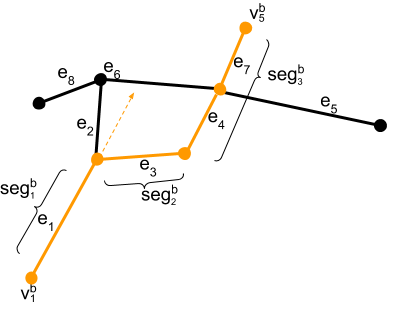
\includegraphics[scale=0.4]{Pictures/ant_segmentMagnitude_case_2.png}
    \end{subfigure}%
    \begin{itemize}
        %\item El criterio de curvatura puede no ser suficiente por si mismo
        \item Comportamiento esperado de la rigidez permite descartar soluciones con cambios demasiado pronunciados entre sus segmentos
    \end{itemize}
\end{figure*}
\end{frame}

%%\subsection{Extracci\'on de informaci\'on para individualizar filamentos}
\begin{frame}{Criterio espec\'ifico para neuronas (OE 1)}
    \begin{itemize}
        \item Se debe validar que los filamentos de una neurona parten del {\bf soma}
        \item  Extracci\'on de informaci\'on: caracter\'isticas geom\'etricas, topol\'ogicas y espaciales
    \end{itemize}
    \begin{columns}
        \begin{column}{0.55\textwidth}
        \centering
        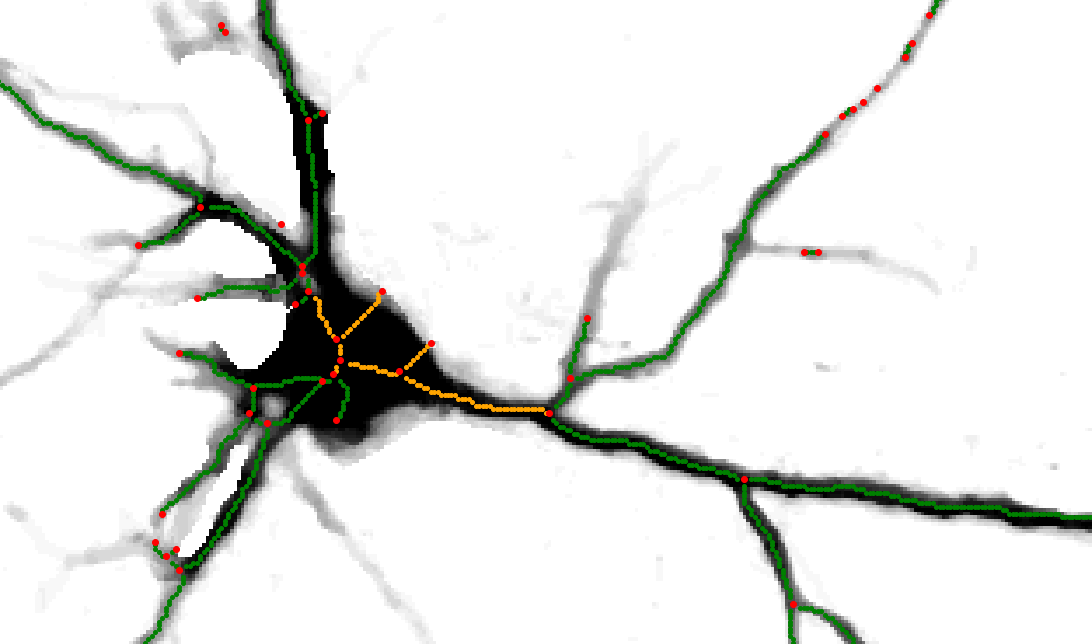
\includegraphics[height=1.7in]{Pictures/Porta183-somaEdges-example2.png}
        \end{column}
        \begin{column}{0.45\textwidth}
            \begin{equation}
                \tau_{ij} \leftarrow
                    \begin{cases}
                     \tau_{ij} \cdot \gamma \text{ si } deg(v^{a}_{n}) = 1,  \\[3ex]
                    
                    \text{0 si } \tau_{ij} \leq 0.25, \\[3ex]
                    \tau_{ij} \quad \text{en otro caso}.
                    \end{cases}
            \end{equation}
        \end{column}
    \end{columns}
    
\end{frame}

% \begin{frame}{Extracci\'on de informaci\'on para individualizar filamentos}
%      \begin{figure*}[h!]
%     \centering
%     \begin{subfigure}[t]{0.48\textwidth}
%         \centering
%         %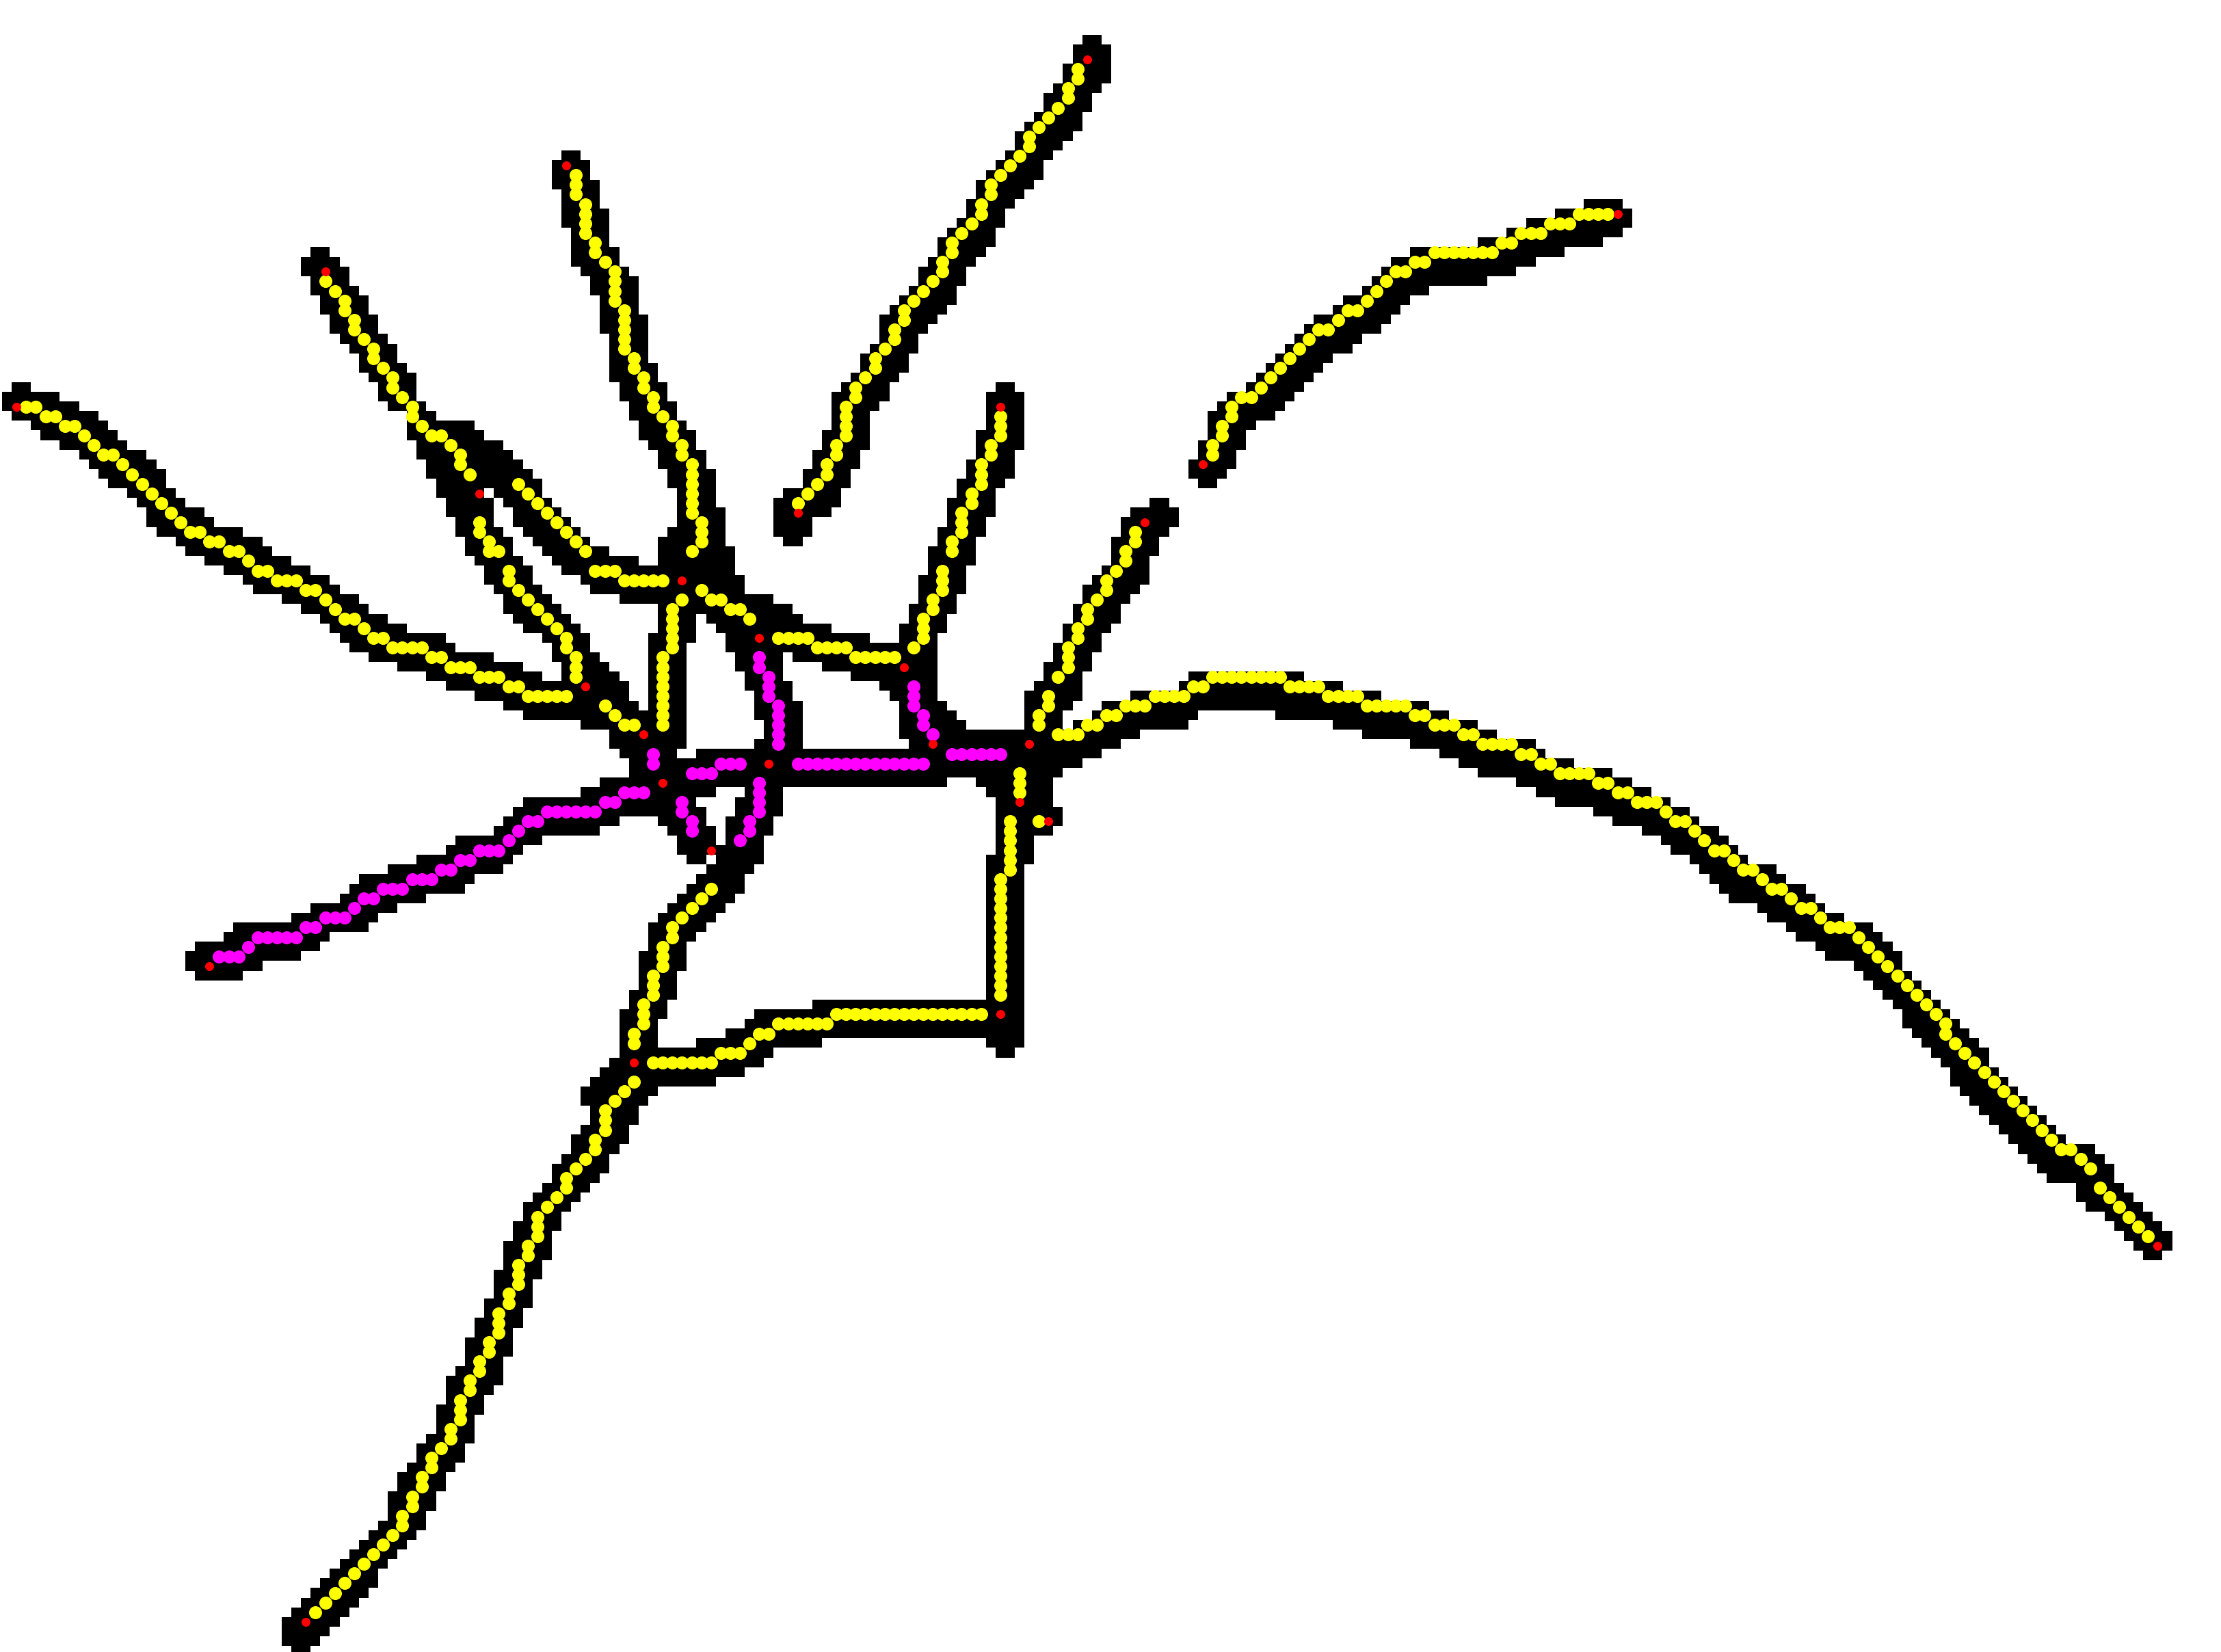
\includegraphics[height=1.5in]{Pictures/50-ROIs-Spinning-Marchantia-somaEdges.png}
%     \end{subfigure}%
%     ~ \hspace{0.1cm}
%     \begin{subfigure}[t]{0.48\textwidth}
%     \centering
%         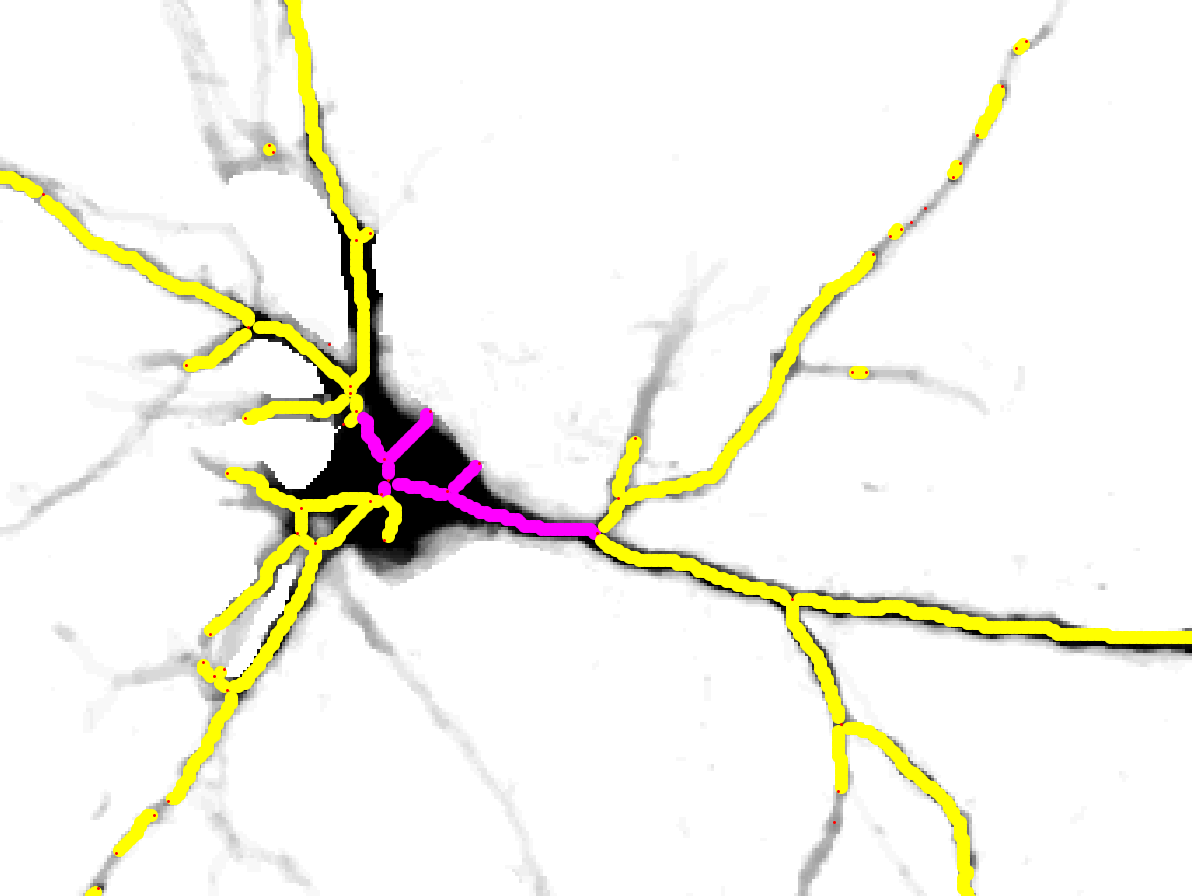
\includegraphics[height=1.5in]{Pictures/Porta18-3a1-somaEdges.png}
%     \end{subfigure}
%     \end{figure*}
%     \begin{itemize}
%         \item Caracter\'isticas geom\'etricas, topol\'ogicas y espaciales
%     \end{itemize}
% \end{frame}
\section{Resultados}



\begin{frame}{Metodolog\'ia}
\begin{itemize}
    \item Par\'ametros principales de las configuraciones utilizadas:
        \begin{itemize}
            \item $\theta$
            \item $Max\_Axial\_Displacement$
            \item Uso de 1 o 3 pasos de la heur\'istica de asignaci\'on inicial
        \end{itemize}
    
    \item 12 Im\'agenes: 2 Sint\'eticas, 7 de Microt\'ubulos en {\it Arabidopsis Marchantia} y 3 de neuronas de rat\'on
    \begin{itemize}
        \item Caso evaluado por 2 expertos
    \end{itemize}
    
    %\item M\'etricas y Medidas:  VI, \'Indice Rand, \'Indice Jaccard
    \item Evaluaci\'on de:
        \begin{itemize}
            \item {\it Precision}, {\it Recall}, F1/F-Measure
            \item N$\degree$ filamentos propuestos y correctos vs {\it ground truth}
        \end{itemize}
\end{itemize}
\end{frame}

\note[itemize]{
    \item Dentro de los par\'ametros disponibles para personalizar el algoritmo propuesto, los principales par\'ametros utilizados en las pruebas fueron el umbral theta, el par\'ametro max axial displacement y el uso parcial o total de la heurística de asignaci\'on inicial
    \item Estos par\'ametros fueron los que mostraron mayor impacto en los resultados
    \item Las pruebas consideraron un total de 12 im\'agenes entre sint\'eticas y reales, con una imagen de microt\'ubulo de planta siendo evaluada por 2 expertos.
    \item La evaluaci\'on se centra en el n\'umero de filamentos propuestos o correctos que indica el algoritmo propuesto. Esta informaci\'on se complementa con las medidas de precision y recall.
    
    %\item (SKIP) N$\degree$ Filamentos Propuestos y Correctos vs {\it Ground Truth}
    
    \item El resultado de la individualización de filamentos para cada imagen, consiste en el promedio de 10 iteraciones del algoritmo propuesto, cambiando en cada ocasión la semilla con la finalidad de explorar el espacio de b\'usqueda desde distintas partes.
}





% \begin{frame}{Im\'agenes Sint\'eticas}

%     \begin{figure*}[h]
%         \centering
%         \begin{subfigure}[t]{0.31\textwidth}
%             \centering
%             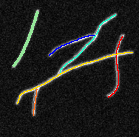
\includegraphics[height=1.3in]{Pictures/Synth-QuantitativeIFS-Fig7_groundTruth.png}
%         \end{subfigure}
%         ~ %\hspace{0.1cm}
%         \begin{subfigure}[t]{0.31\textwidth}
%             \centering
%             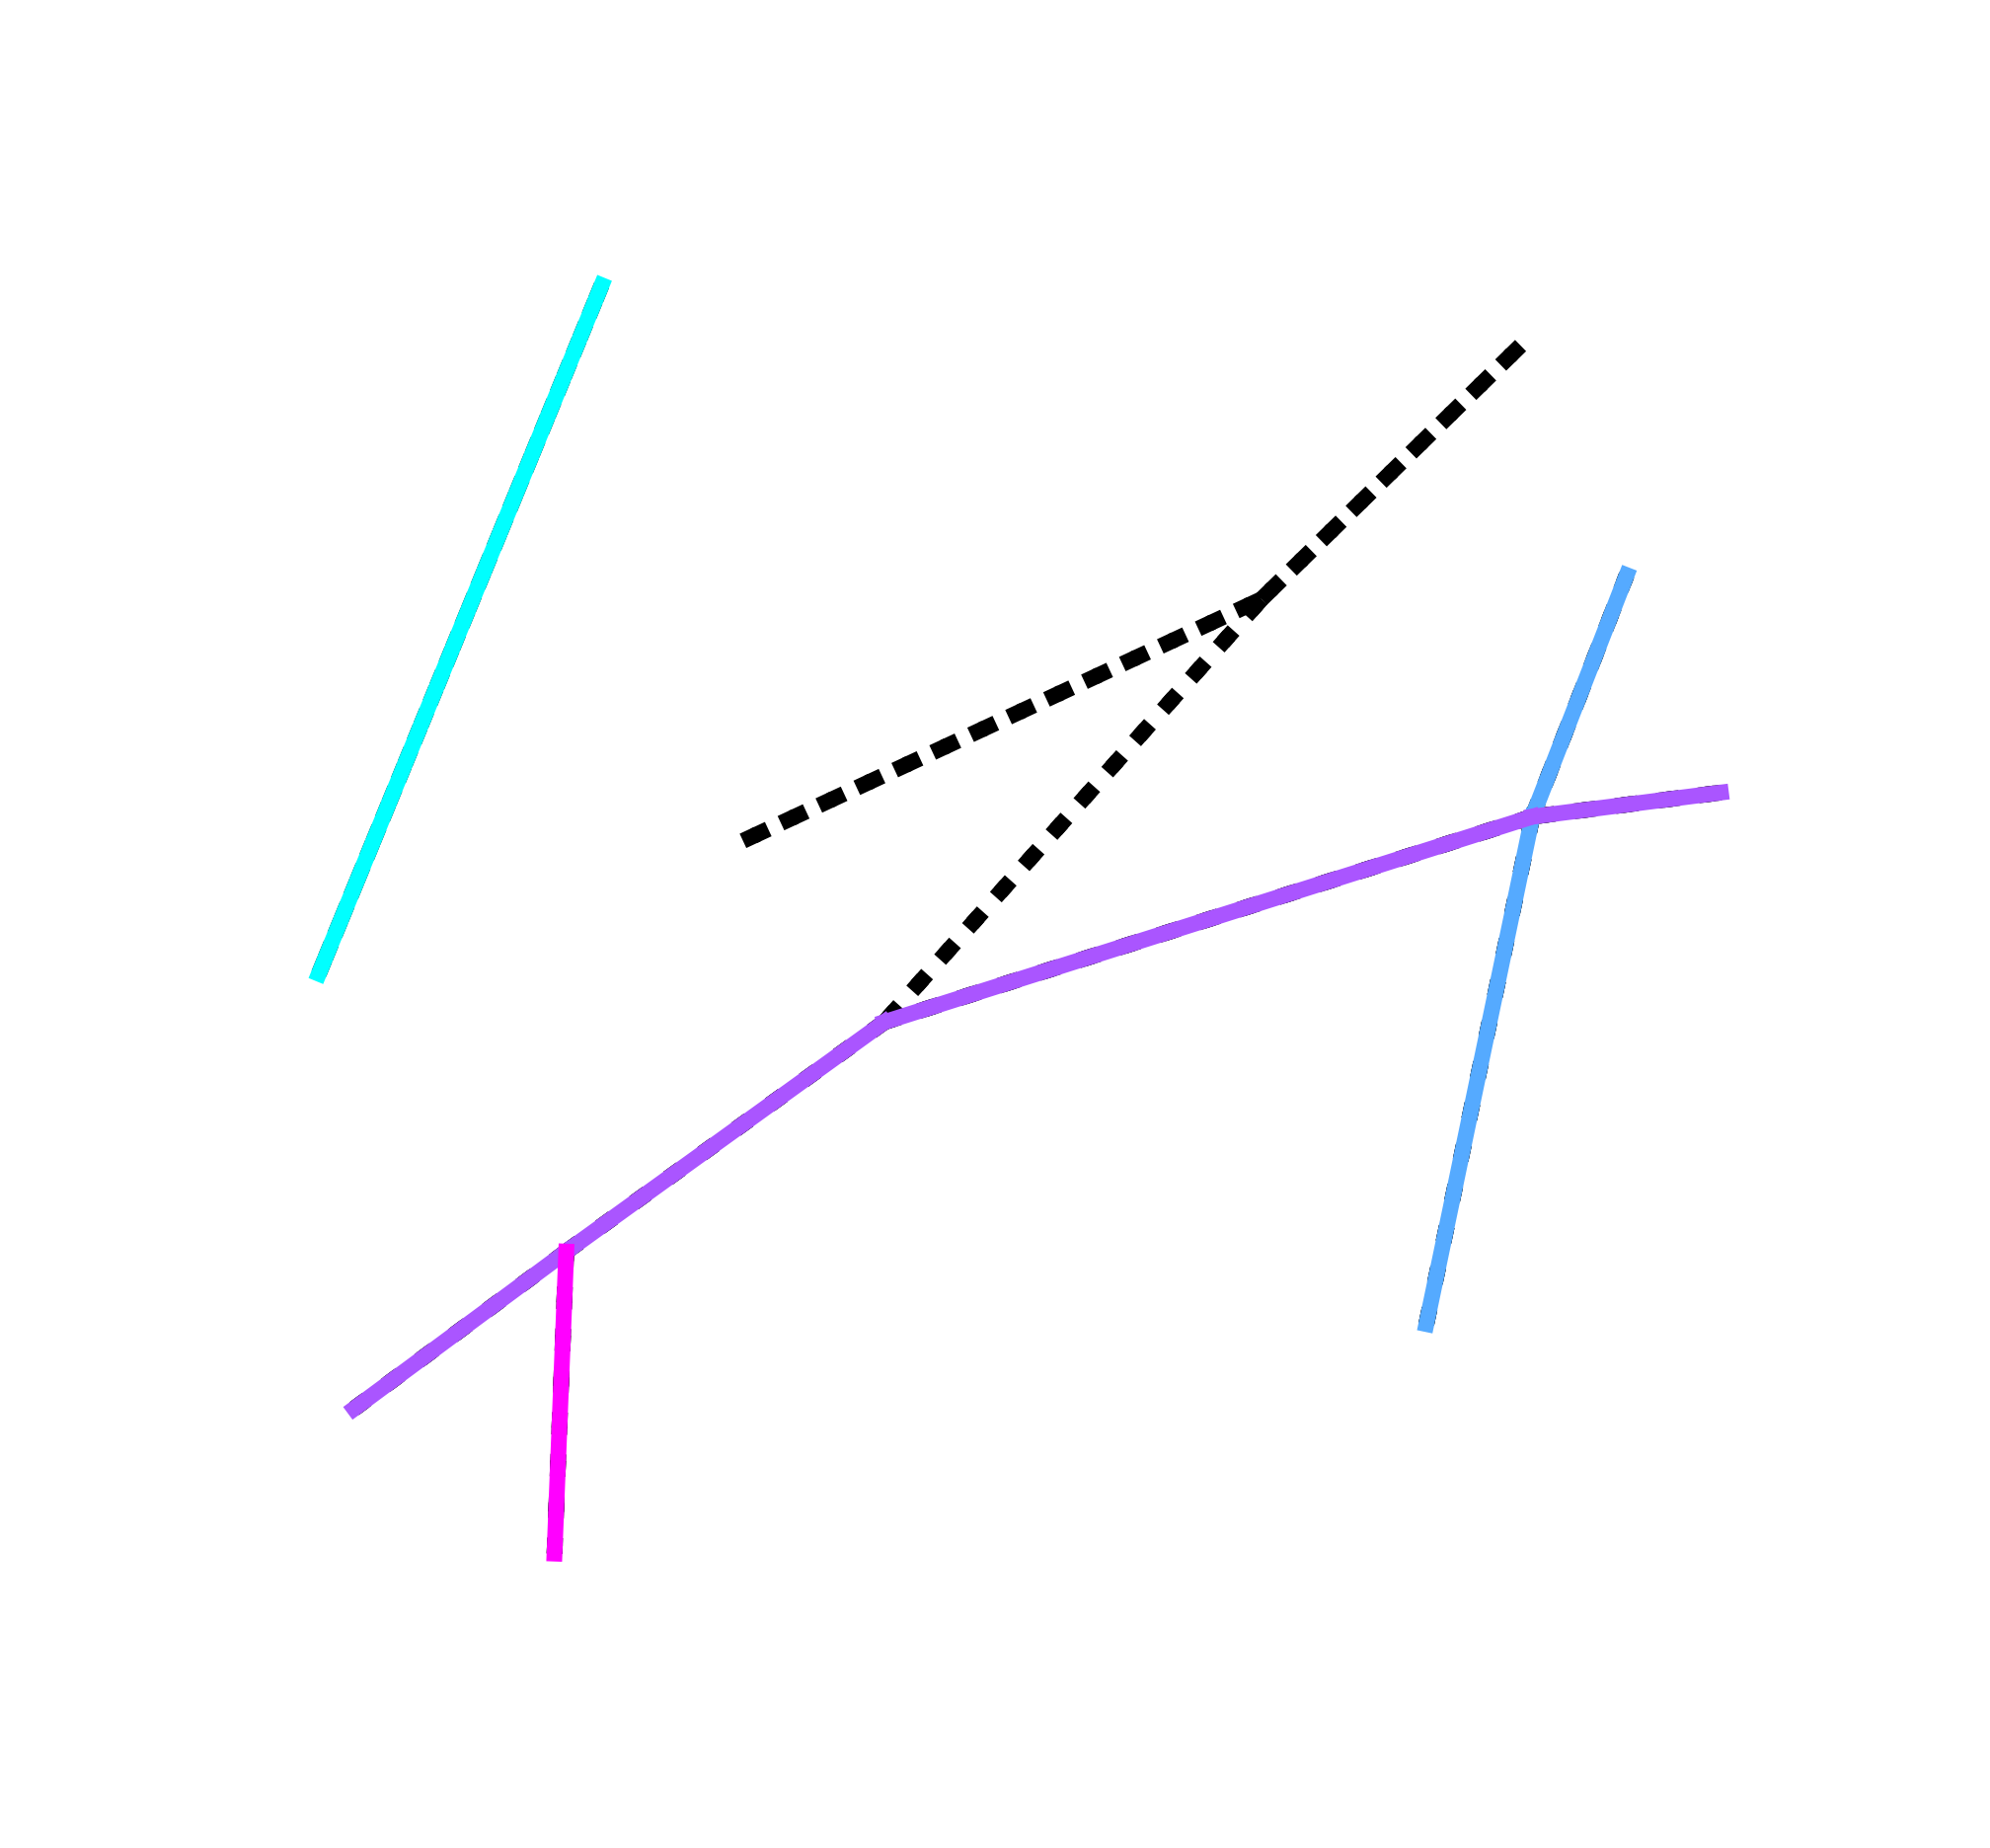
\includegraphics[height=1.3in]{Pictures/QFS7-DeFiNeExactMatch-30.png}
%         \end{subfigure}
%         ~
%         \begin{subfigure}[t]{0.31\textwidth}
%             \centering
%             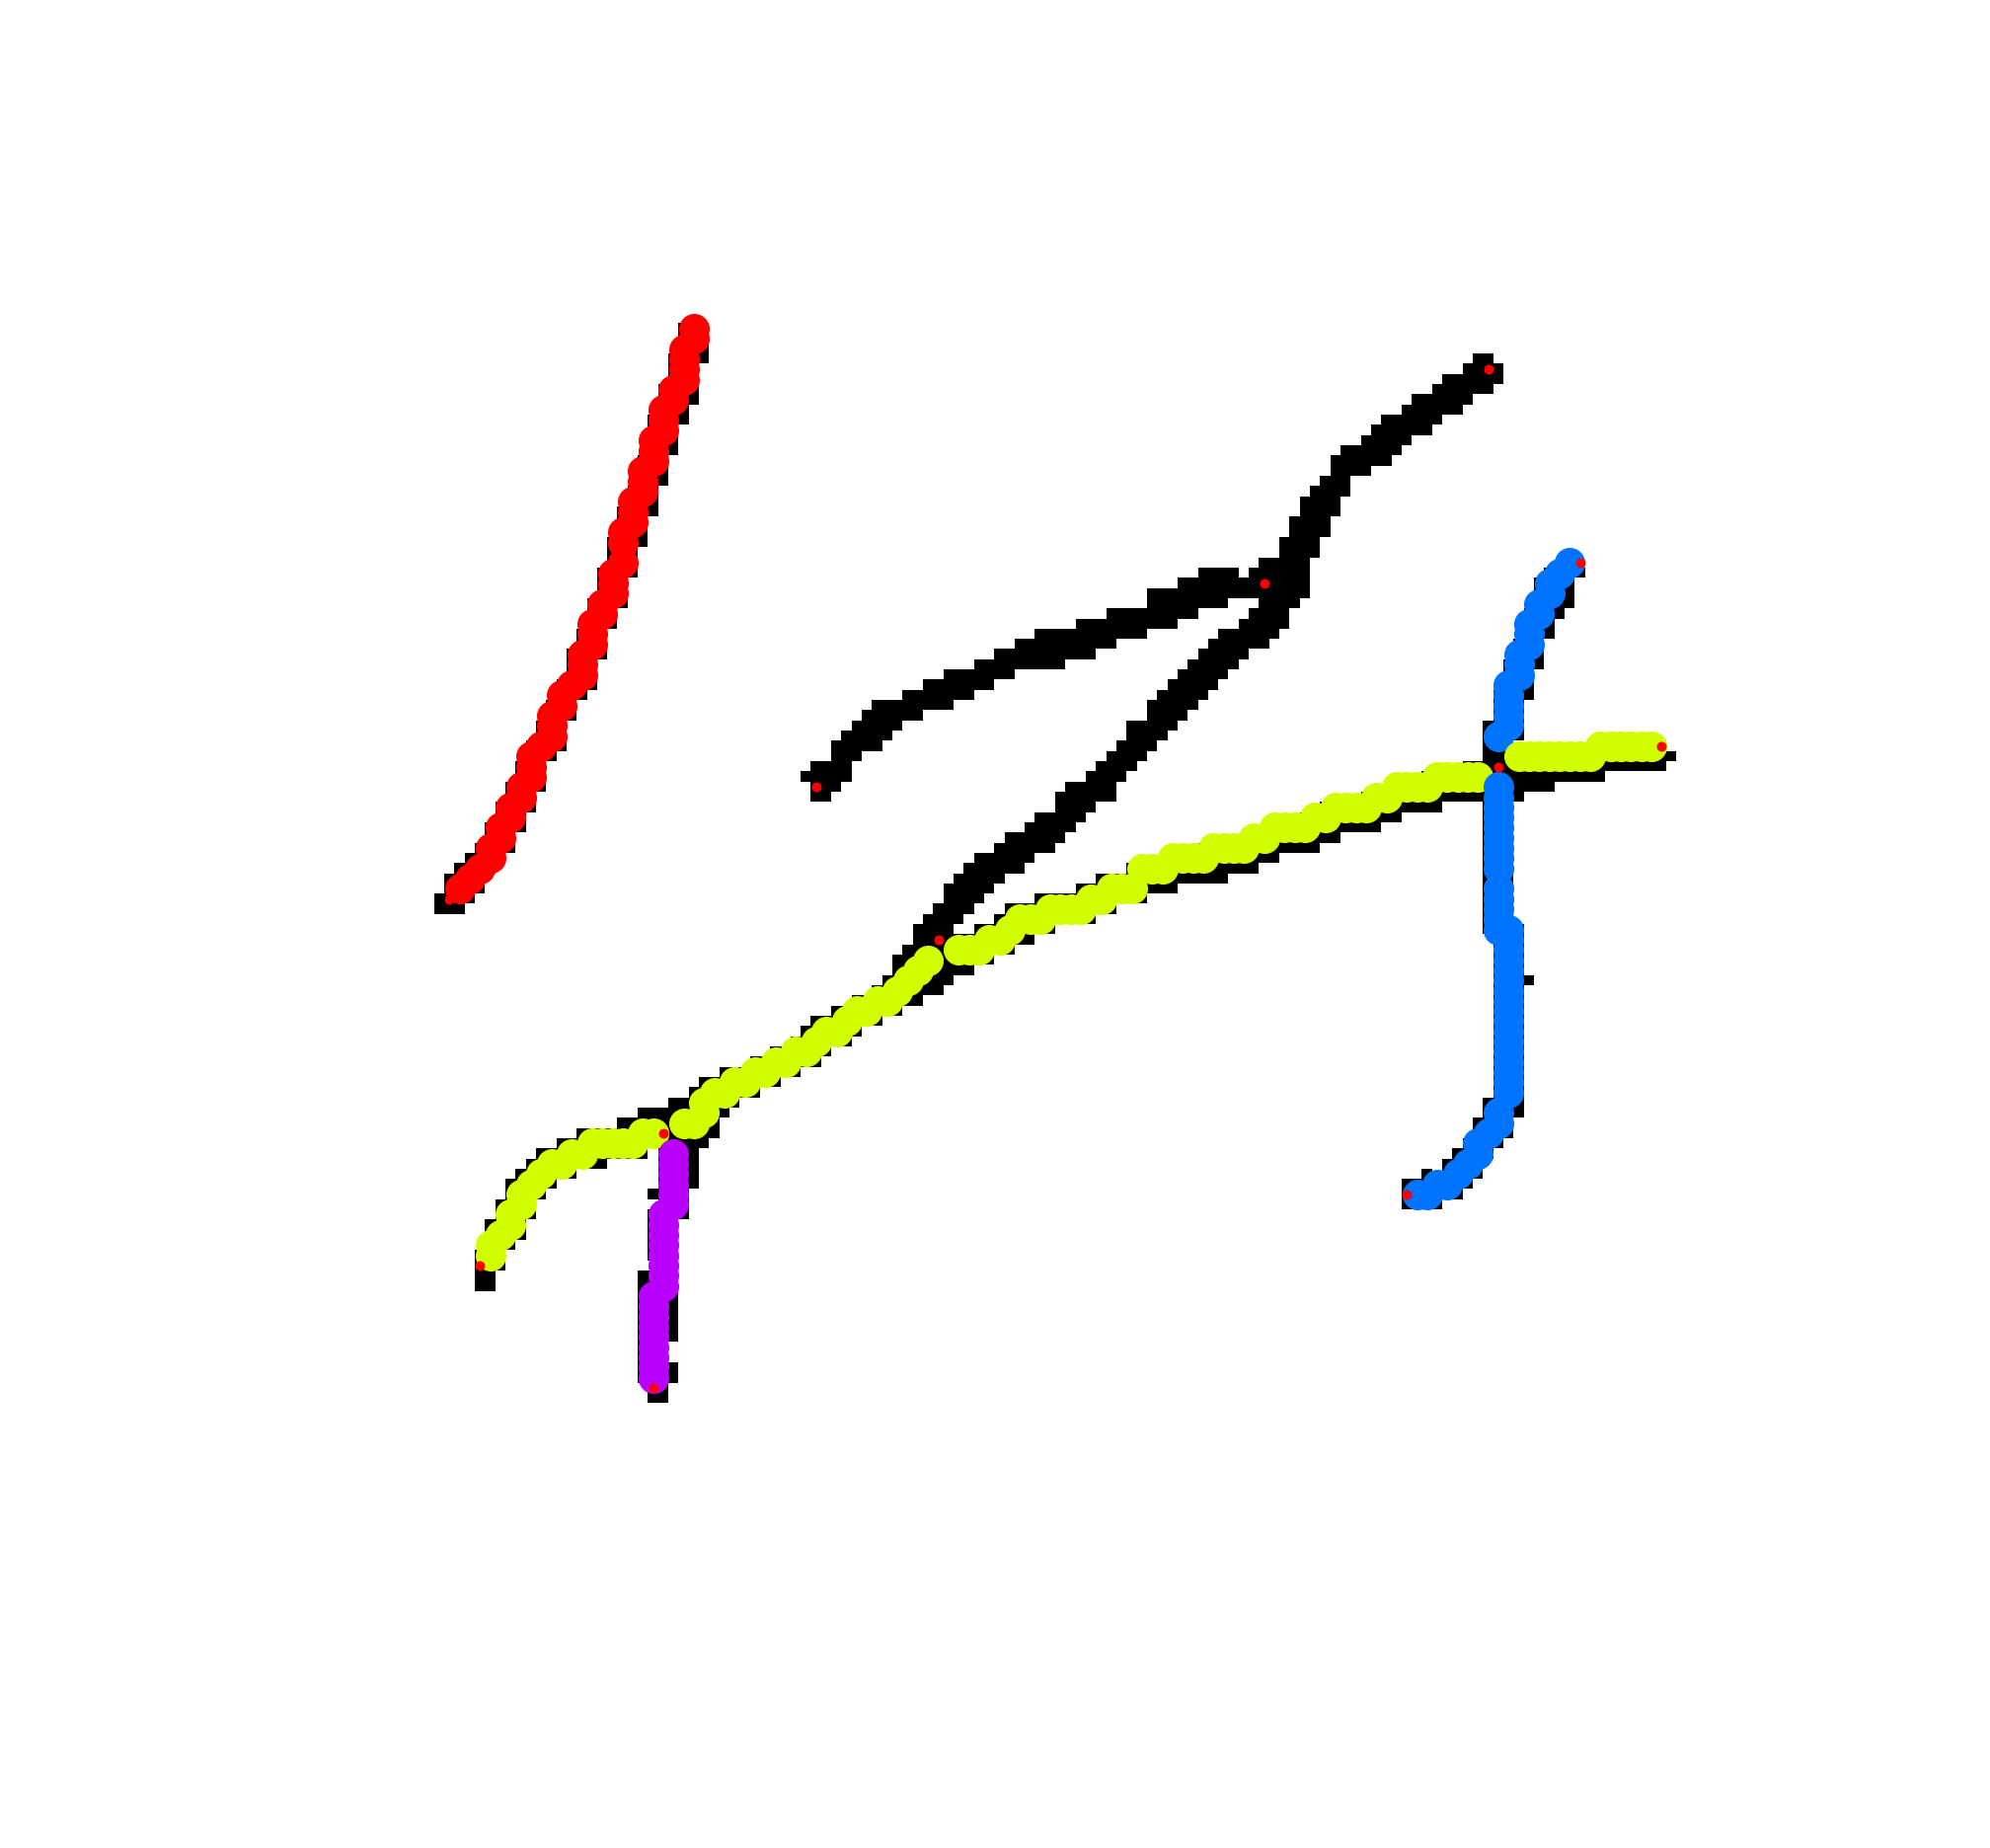
\includegraphics[height=1.3in]{Pictures/Synth-QuantitativeIFS-Fig7-phil-s1271-v056-exactMatch-antLabeled.png}
%         \end{subfigure}
%     \end{figure*}
    
% \resizebox{\textwidth}{!}{
%         %\footnotesize
%         \begin{tabular}{|c|c|c|c|c|c|c|c|c|c|c|c|c|}
%         \hline
%             Config & Iters & P & P* & R & R* & F1 & F1* & C/P & C/P* & C/GT & C/GT* & T[s]\\ \hline
%              DeFiNe 30\textdegree  & 1 & 0.72 & - & 0.47 & - & 0.57 & - & 4/6 & - & 4/6 & - & 2.3 \\
%              DeFiNe 60\textdegree & 1 &0.63 & - & 0.58 & - & 0.60 & - & 3/5 & - & 3/6 &- & 2.3\\
%             AP MT-P & 5 & 0.51 & 0.57 & 0.32 & 0.57 & 0.39 & 0.57 & 3/6.2 & 3/5 & 3/6 & 3/6 & 0.3\\
%             %Mejor Iteraci\'on P1 & 0.5714 & 0.5714 & 0.5714 & 3/5 &  & 0.3135 \\
%             AP S1 & 5 & 0.68 & 0.87 &0.57 & 1 & 0.62 & 0.93 & 4/5.8 & 4/5 & 4/6 & 4/6 & 0.2\\
%             % {\bf Mejor Iteraci\'on P2} & 0.875 & 1 & 0.9333 & 4/5 & 4/6 & 0.3073\\
%              \hline
%         \end{tabular}
%     }
% \end{frame}

\begin{frame}{Im\'agenes Sint\'eticas (OE 4)}
    \vspace{-0.6cm}
    \begin{columns}
        \begin{column}{0.31\textwidth}
        
            \begin{figure}
                \centering
                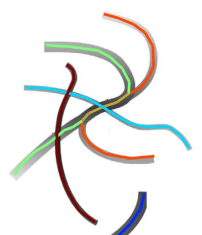
\includegraphics[height=1.3in]{Pictures/define-weighted-4-groundTruth.png}
                \caption{Ground Truth}
            \end{figure}
        \end{column}
        \begin{column}{0.31\textwidth}
        %\vspace{-1cm}
            \begin{figure}
                \centering
                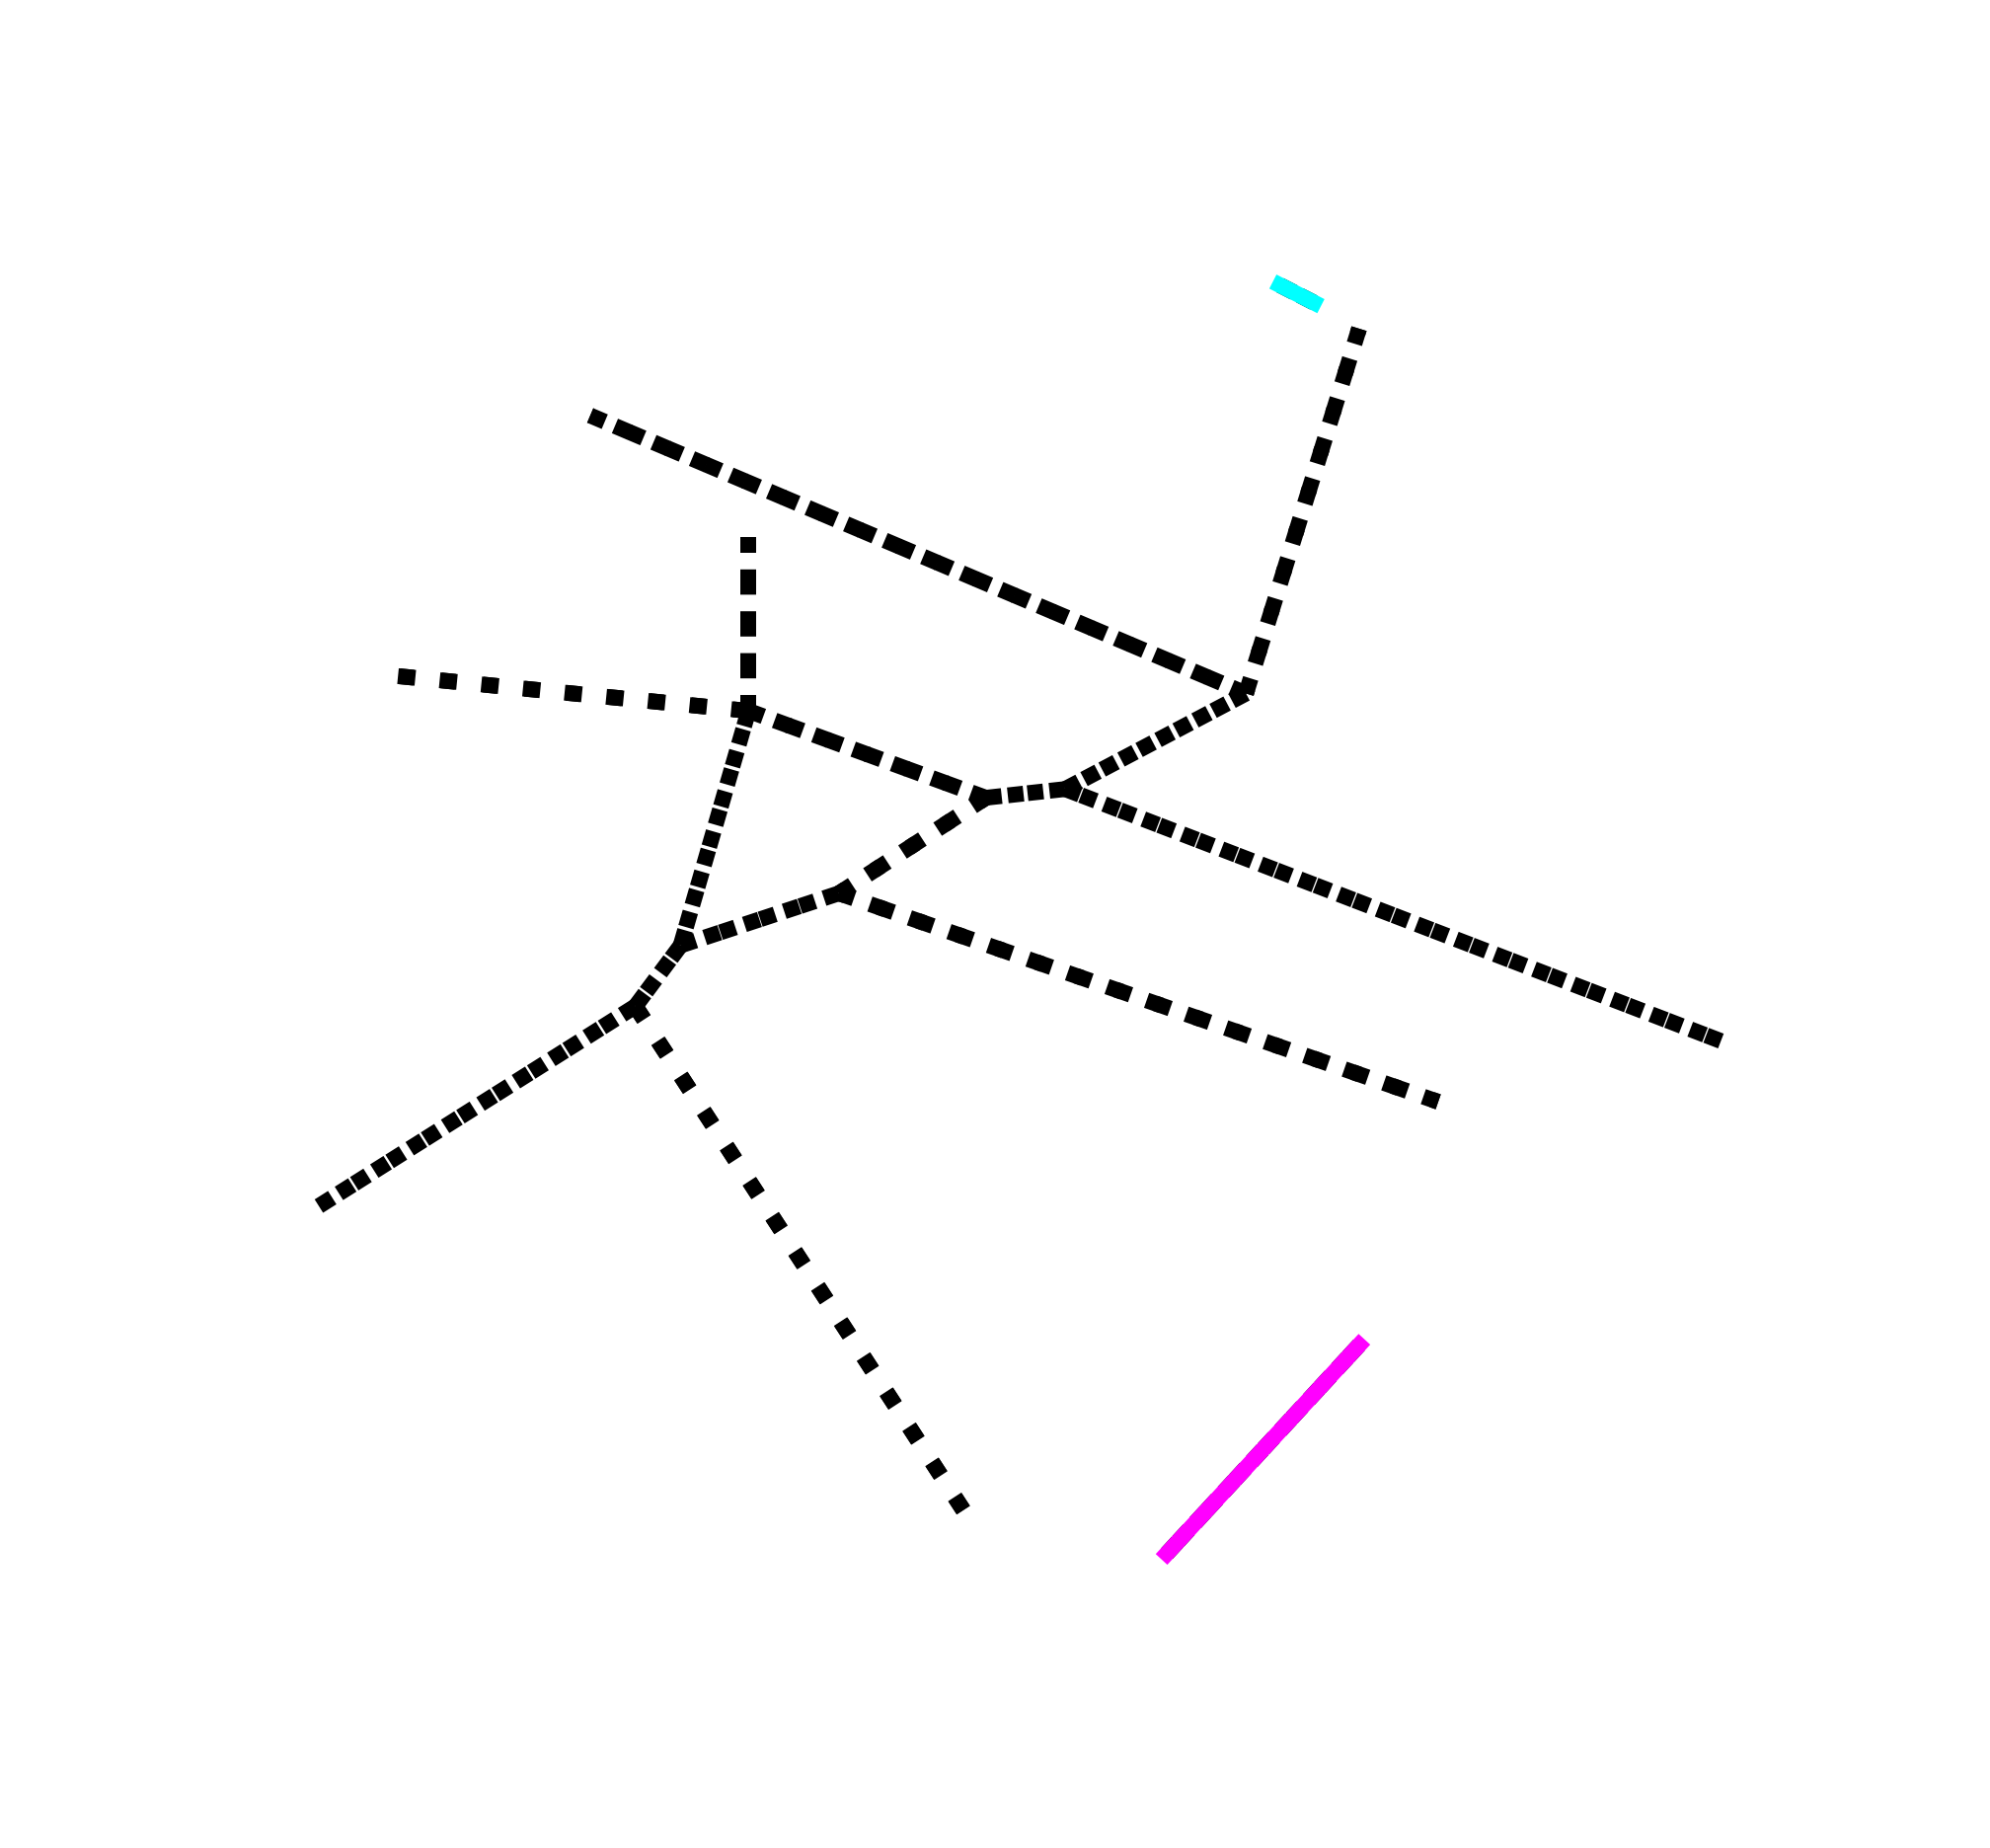
\includegraphics[height=1.3in]{Pictures/defineFig1b-DeFiNeExactMatch-30.png}
                \caption{DeFiNe 30\textdegree}
            \end{figure}
        \end{column}
        \begin{column}{0.31\textwidth}
        %\vspace{-1cm}
            \begin{figure}
                \centering
                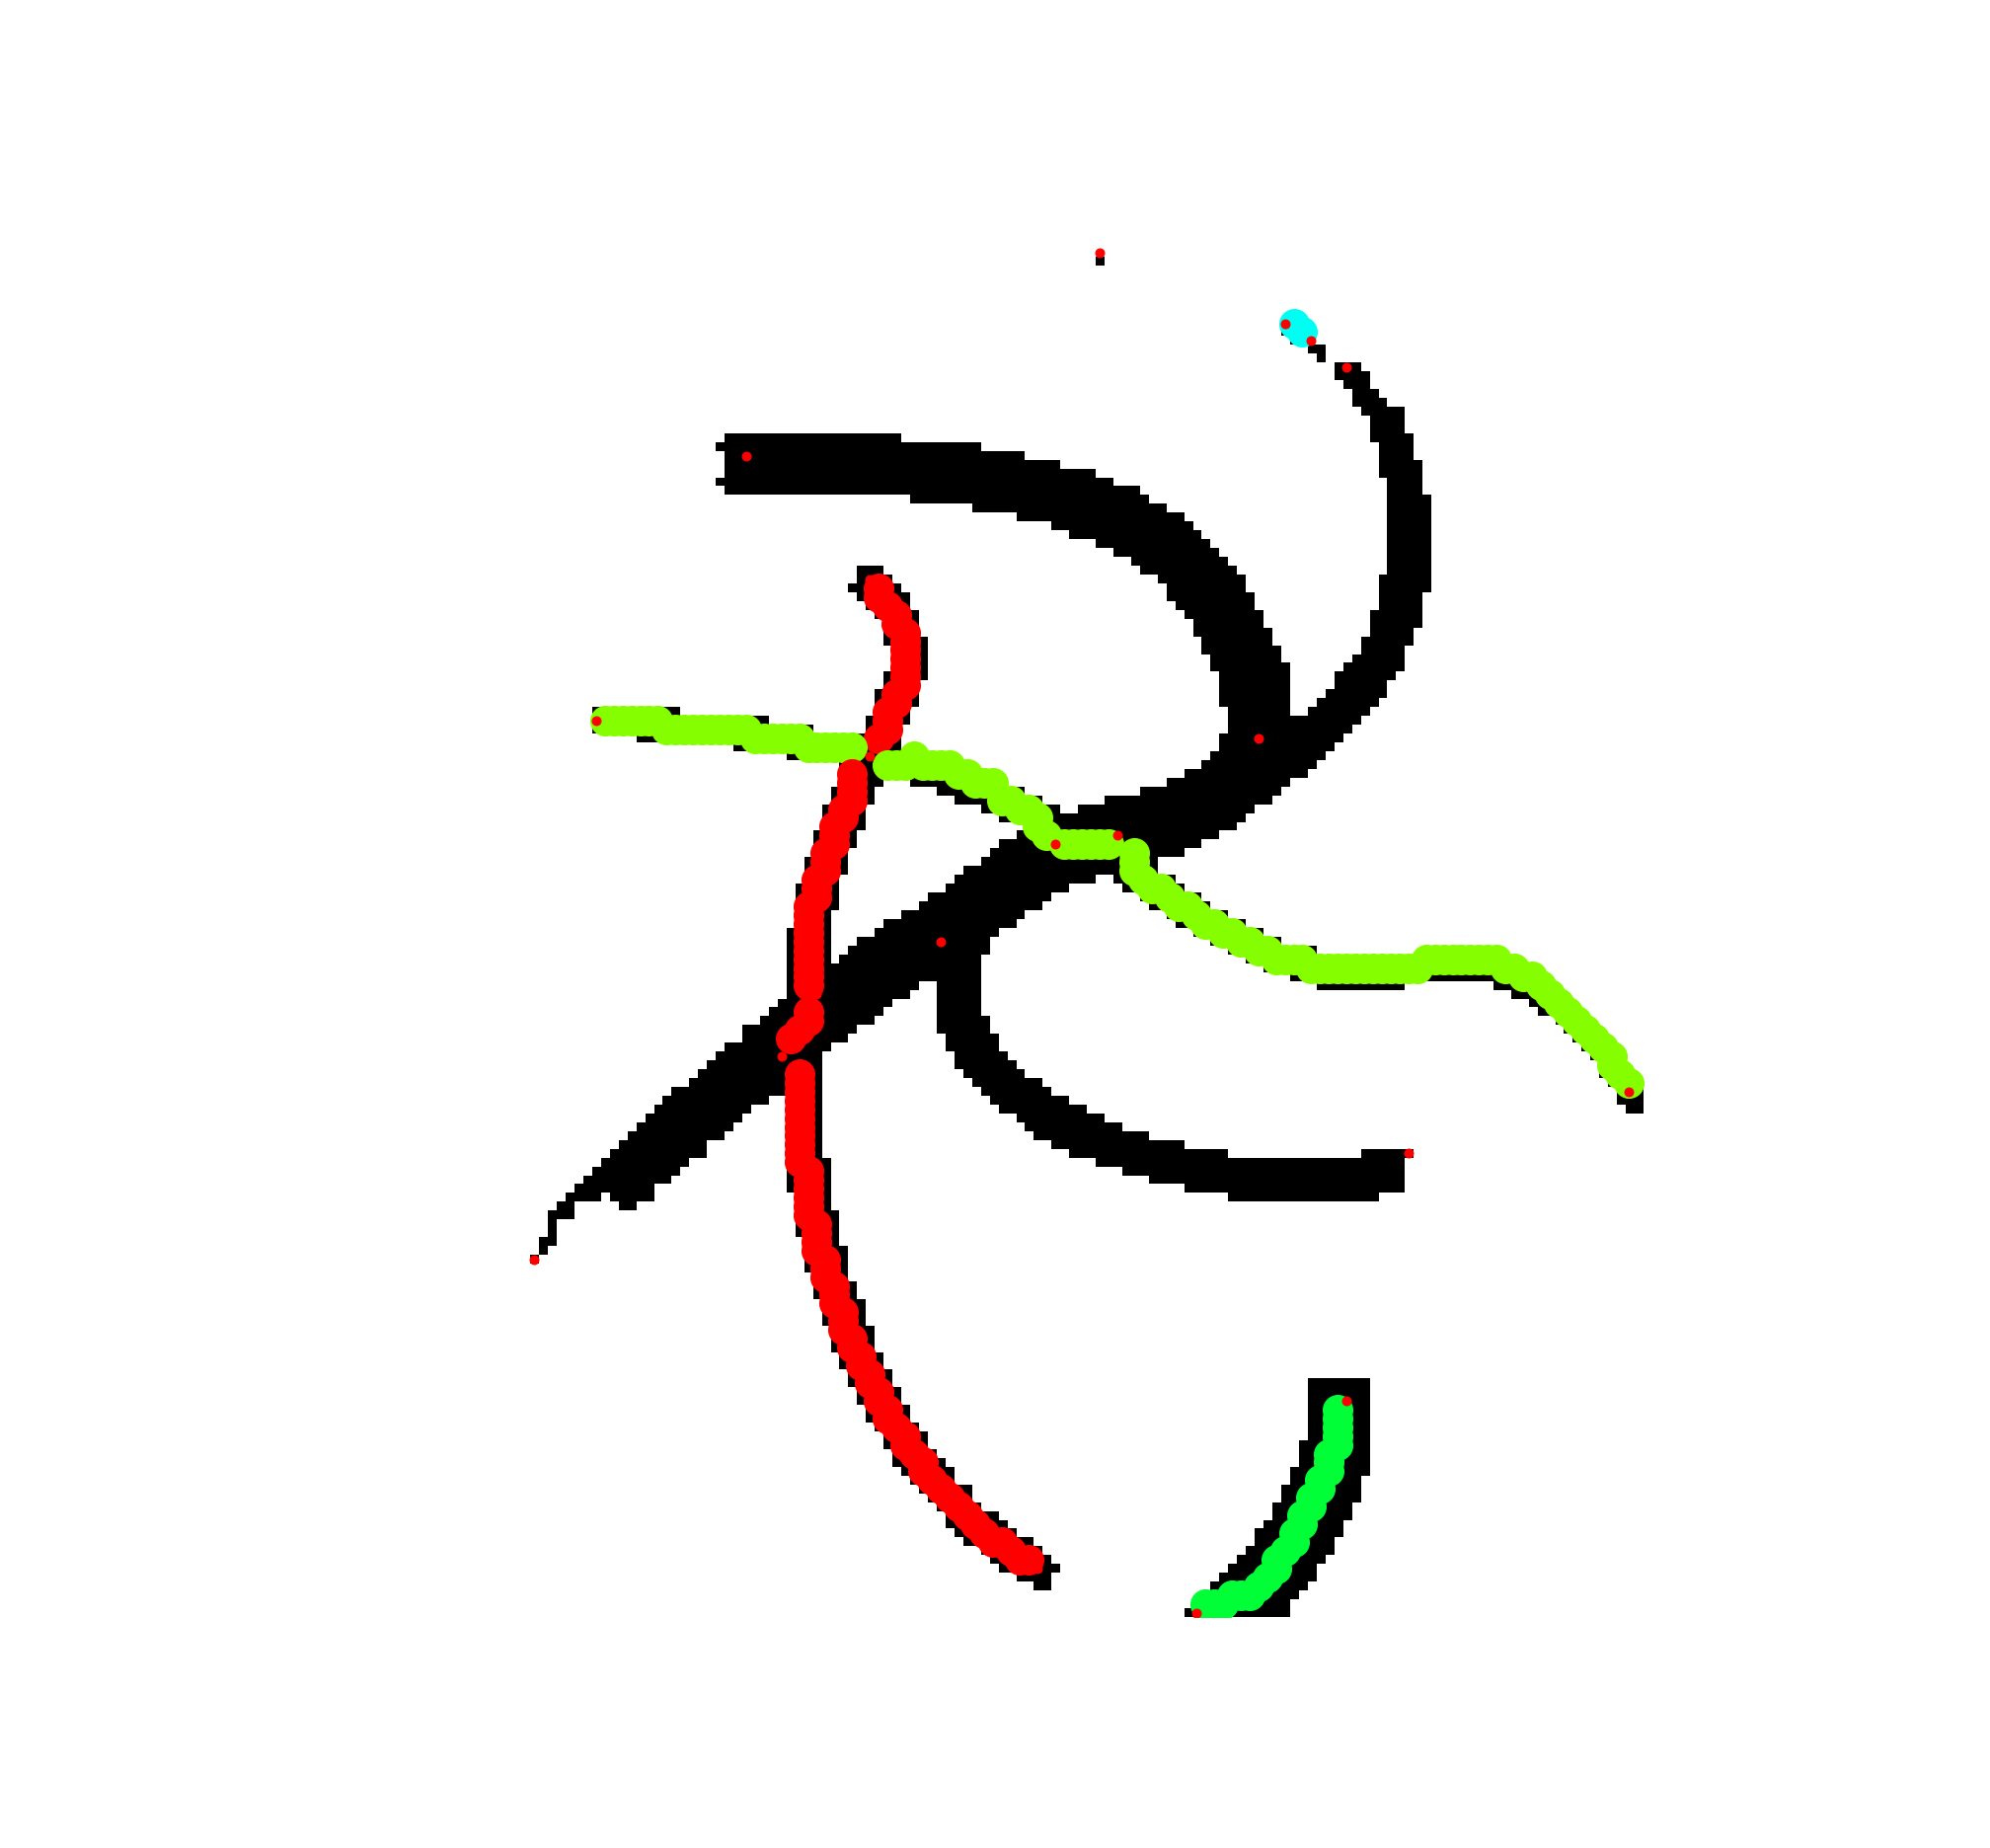
\includegraphics[height=1.3in]{Pictures/define-weighted-4-phil-s3389-v056-exactMatch-antLabeled.png}
                \caption{AP S2}
            \end{figure}
        \end{column}
    \end{columns}

    \vspace{-0.3cm}
    \begin{table}[h]
    \resizebox{\textwidth}{!}{
        \begin{tabular}{|c|c|c|c|c|c|c|c|c|c|c|c|c|}
        \hline
        Config & Iters & P & P* & R & R* & F1 & F1* & C/P & C/P* & C/GT & C/GT* & T[s] \\ \hline
        DeFiNe 30\textdegree & 1 & 0.33 & - & 0.18 & - & 0.23 & - & 2/11 & - & {\bf 2/5} & - & 2.8 \\
        DeFiNe 60\textdegree & 1& 0.23 & - & 0.25 & - & 0.24 & - & 2/7 & - & 2/5 & - & 3.6\\
        AP MT-P & 5 & 0.34 & 0.35 & 0.27 & 0.28 & 0.3 & 0.31 & 3/9.2 & 3/9 & 3/6 & 3/6 & 0.3\\
        AP S2 & 5 & 0.32 & 0.33 & 0.25 & 0.31 & 0.28 & 0.32 & 4/8.6 & 4/9 & {\bf 4/6} & 4/6 & 0.3\\
            \hline
        \end{tabular}
    }
    \caption{Grafo de 17 aristas \\(*) indica el mejor resultado de las 5 iteraciones.}
    \end{table}
\end{frame}

\begin{frame}{Muestra MT-A Microt\'ubulo (OE 4)}
\vspace{-1cm}
    \begin{columns}
        \begin{column}{0.22\textwidth}
            \begin{figure}
                \centering
                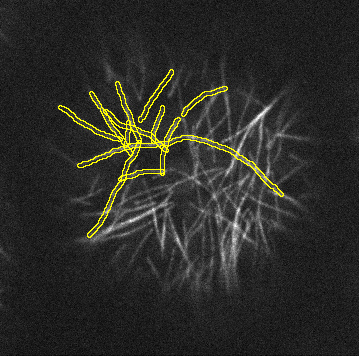
\includegraphics[height=1.3in]{Pictures/SPINNING-DISK-MARCHANTIA-rois-unlabeled.png}
                \caption{Imagen Original}
            \end{figure}
        \end{column}
        \begin{column}{0.22\textwidth}
            \begin{figure}
                \centering
                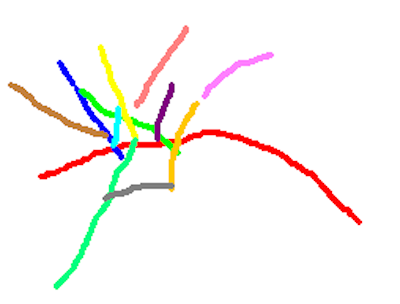
\includegraphics[height=1.3in]{Pictures/50-ROIs-Spinning-Marchantia-solved-rot-unlabeled.png}
                \caption{Ground Truth}
            \end{figure}
        \end{column}
        \begin{column}{0.22\textwidth}
            \begin{figure}
                \centering
                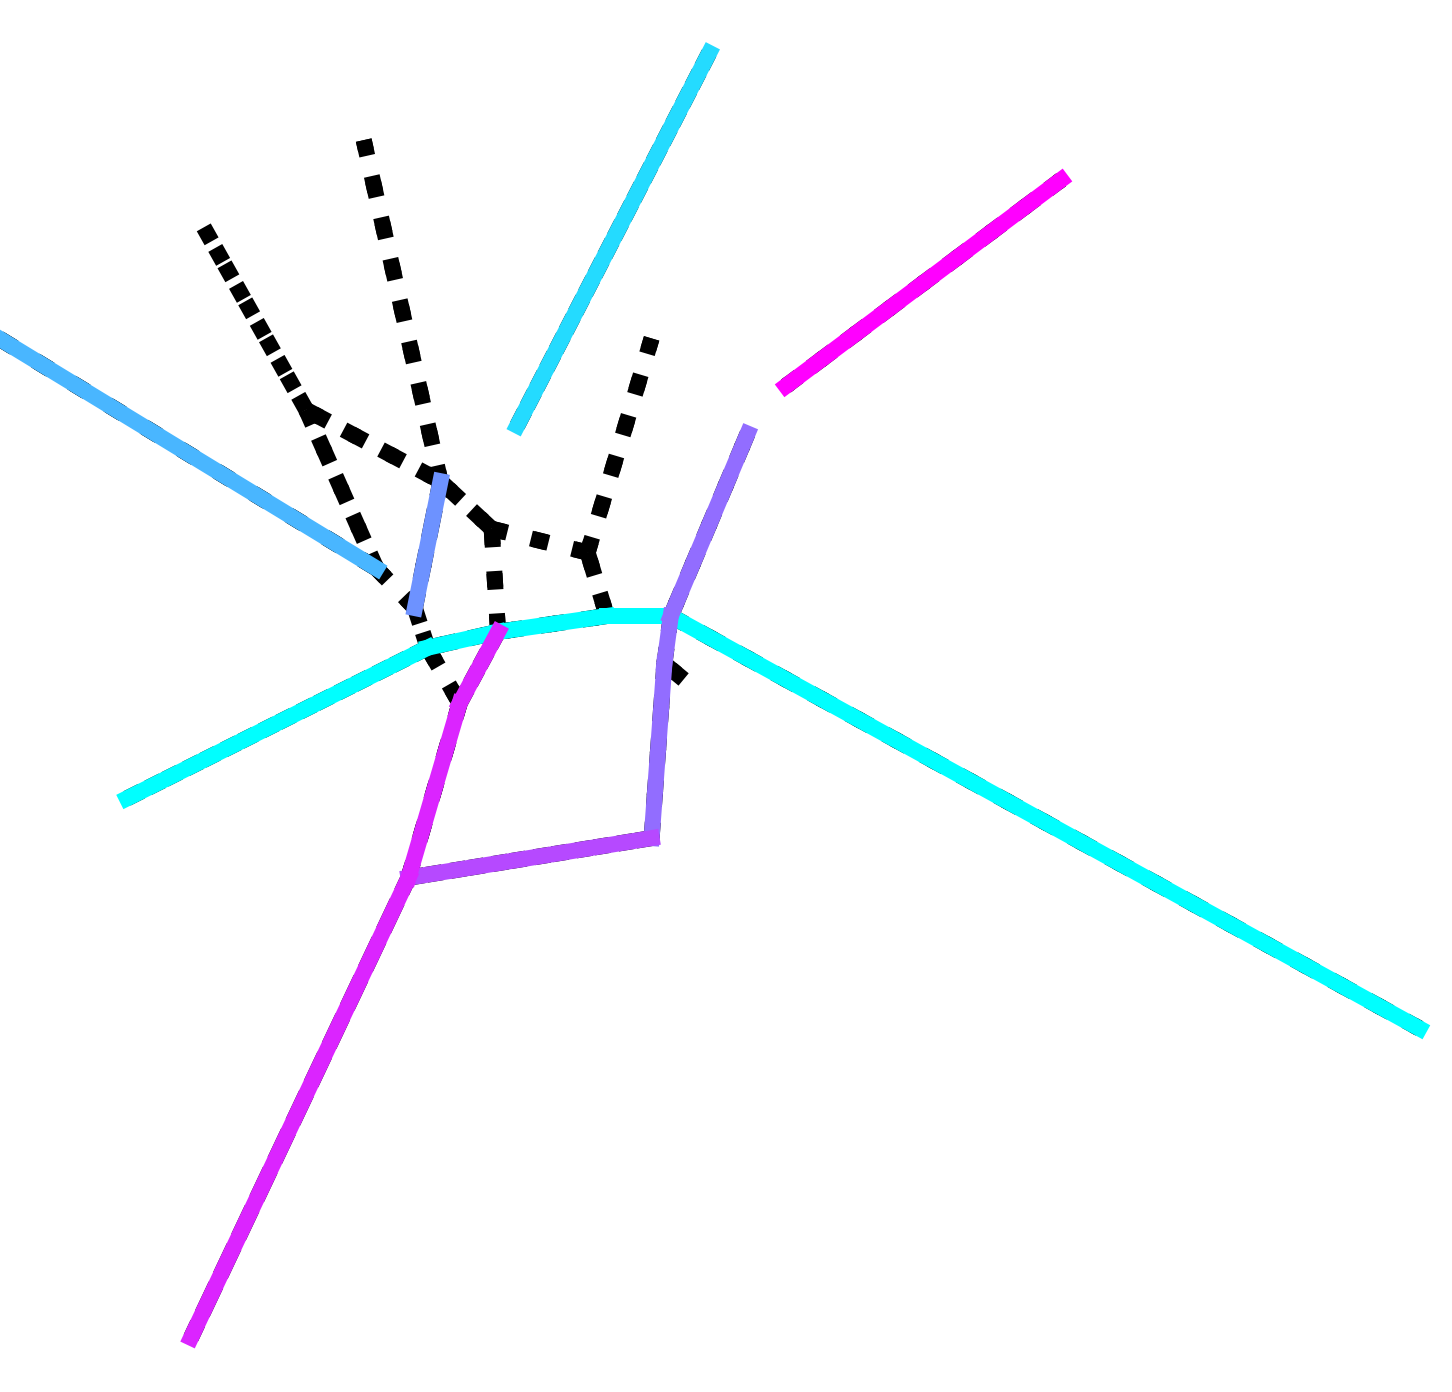
\includegraphics[height=1.3in]{Pictures/50-ROIs-Spinning-Marchantia-DeFiNeExactMatch-30.png}
                \caption{DeFiNe 30\textdegree}
            \end{figure}
        \end{column}
        \begin{column}{0.22\textwidth}
            \begin{figure}
                \centering
                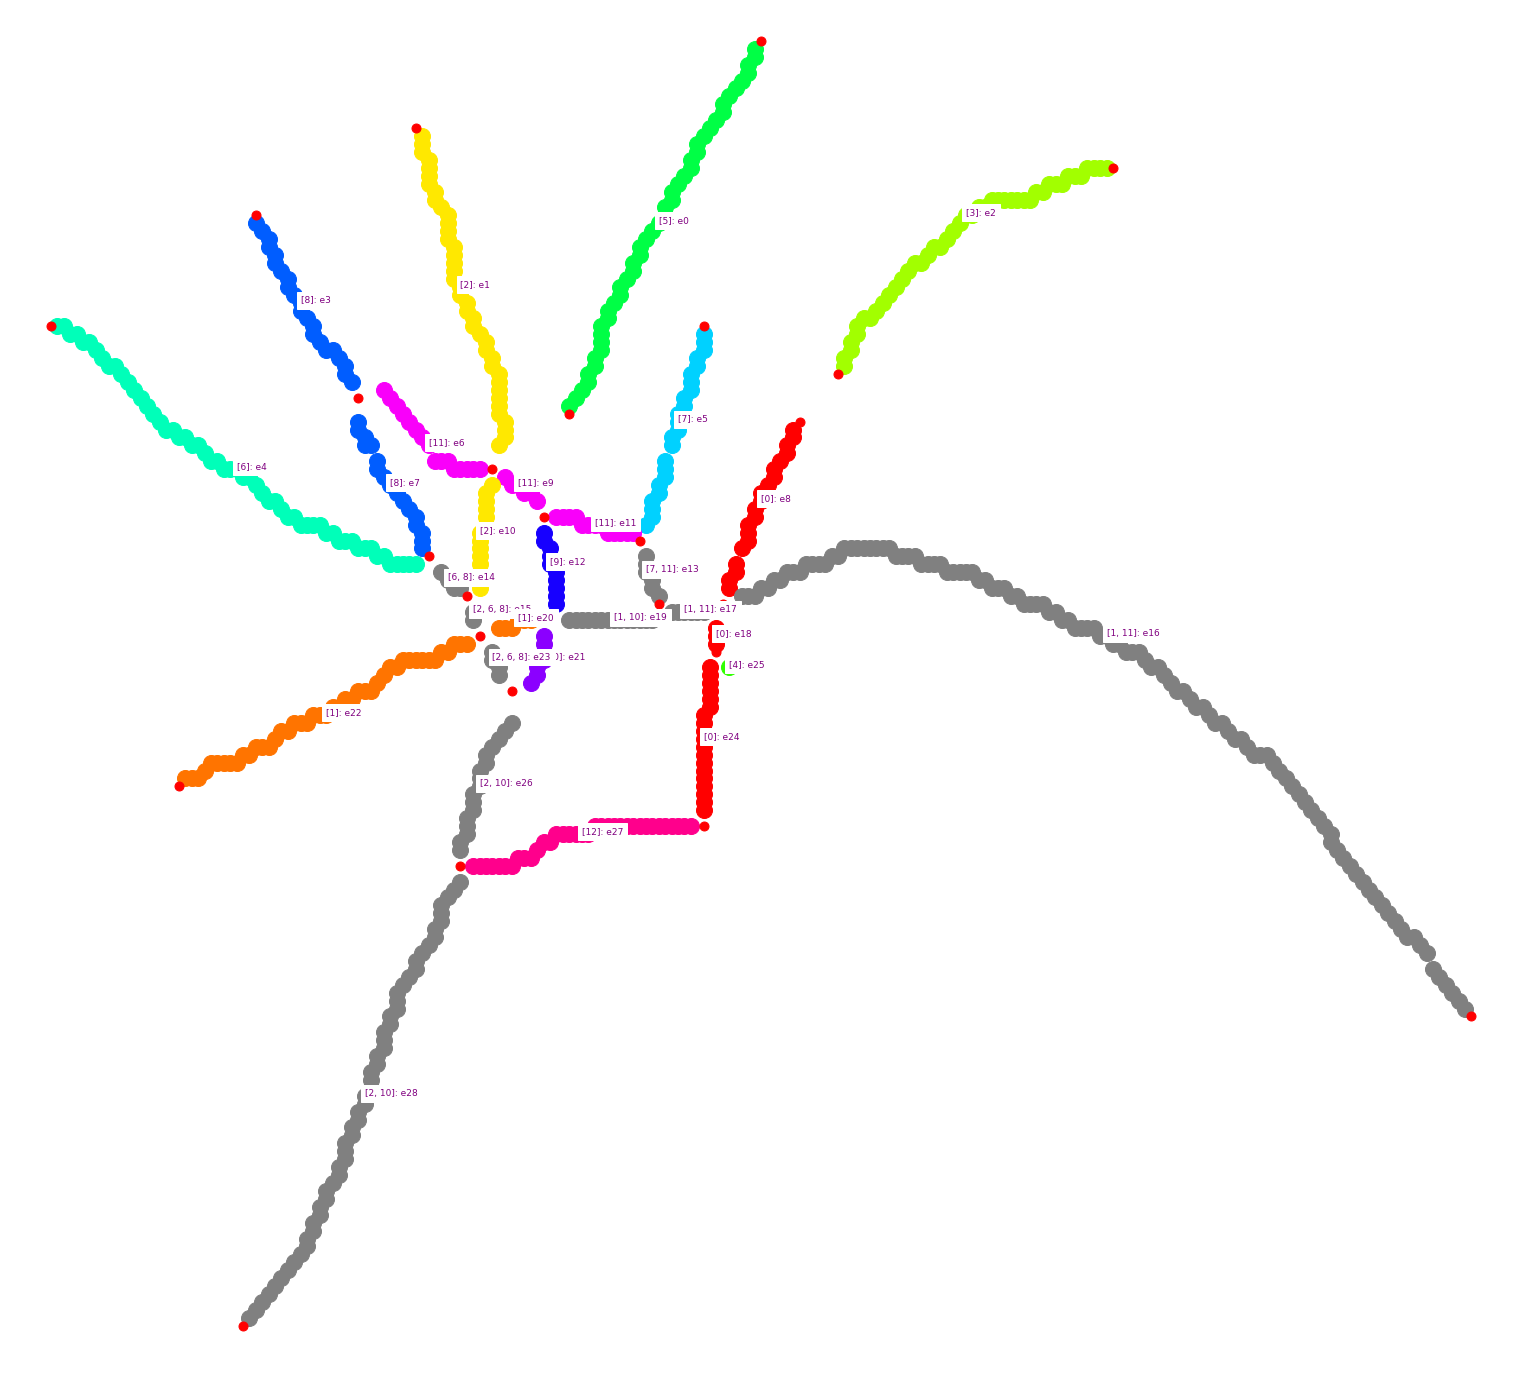
\includegraphics[height=1.3in]{Pictures/50-ROIs-Spinning-Marchantia-phil-s10-v05-nobg-antLabeled.png}
                \caption{AP S2}
            \end{figure}
        \end{column}
    \end{columns}

    \begin{table}[h]
    \resizebox{\textwidth}{!}{
        \begin{tabular}{|c|c|c|c|c|c|c|c|c|c|c|c|c|}
        \hline
              Config & Iters & P & P* & R & R* & F1 & F1* & C/P & C/P* & C/GT & C/GT* & T[s] \\ \hline
             DeFiNe 30\textdegree & 1 & 0.65 & - & 0.45 & - & 0.53 & - & 8/16 & - & {\bf 8/12} & - & 4.1 \\
             DeFiNe 60\textdegree & 1& 0.28 & - & 0.21 & - & 0.24 & - & 3/12 &- & 3/12 & - & 3.6\\
            AP MT-P & 5 & 0.44 & 0.45 & 0.34 & 0.35 & 0.38 & 0.4 & 7.2/12.4 & 8/13 & 7.2/12 & {\bf 8/12} & 0.3\\
             \hline
        \end{tabular}
        }
    \caption{Grafo de 29 aristas \\(*) indica el mejor resultado de las 5 iteraciones}
    \end{table}
\end{frame}

\begin{frame}{Neuronas de rat\'on (OE 4)}
%\vspace{-1cm}
    \resizebox{\textwidth}{!}{
        \begin{tabular}{|c|c|c|c|c|r|c|}
        \hline
             Muestra & Algoritmo & Fil. Propuestos & {\it GT} &\% Asignaci\'on & Tiempo[s] & N\textdegree~ Aristas\\
             \hline
             \multirow{3}{*}{N1}& DeFiNe 30\textdegree & 246 & \multirow{3}{*}{24} &100 & 1514.6 & \multirow{3}{*}{414} \\
                    & DeFiNe 60\textdegree & 192 && 100 & 15573.7 &\\
                    & AP N Promedio & 59 && 53.7 & 32.5 &\\ \hline
            \multirow{3}{*}{N2}& DeFiNe 30\textdegree & 113 & \multirow{3}{*}{29} & 100 & 82.2 & \multirow{3}{*}{161}\\
                    & DeFiNe 60\textdegree & 85 && 100 & 456.4 &\\
                    & AP N Promedio & 34.8 && 59.3 & 4.9 &\\ \hline
            N3 & AP N Promedio & 17.4 & 14 & 57.8 & 4.2 & 67\\ \hline
        \end{tabular}
    }
    \vspace{0.5cm}
    \begin{itemize}
        \item \% Asignaci\'on debe estar relacionado a la calidad de la informaci\'on, evitando asignar s\'olo por cumplir con el modelo
        \item N\textdegree~ Fil. Prop. refleja acotamiento del espacio de b\'usqueda
    \end{itemize}
\end{frame}

\note[itemize]{
\small
  \item En las neuronas de raton, las pruebas ejecutadas con DeFiNe presentan cantidades de filamentos propuestos 2 a 6 veces mayores que el n\'umero de filamentos individualizados por un experto. Este comportamiento puede atribuirse a la obligaci\'on que DeFiNe tiene de asignar todas las aristas al menos a un filamento. En comparaci\'on, el algoritmo propuesto al tener mayor flexibilidad, asigna en promedio un 57\% de las aristas a filamentos.
  
  \item Adicionalmente, los tiempos de ejecuci\'on de las pruebas con DeFiNe son sustancialmente mayores, encontr\'andose en el rango de los minutos a las 4 horas, dependiendo de los par\'ametros utilizados. Lo anterior puede asociarse al n\'umero de aristas que las muestras de neurona tienen en su respectivo grafo
  
  \item En cuanto al algoritmo propuesto, a pesar de ejecutar todas las evaluaciones en tiempos menores a 40 segundos, las individualizaciones correctas son bajas, mientras que el n\'umero de filamentos propuestos se acerca a la cantidad de filamentos individualizados manualmente por un experto, exceptuando el caso de la Muestra N1.
  
  \item  Es posible asociar un comportamiento razonable del n\'umero de filamentos propuestos con la restricci\'on especial para neuronas considerada dentro de las penalizaci\'on de anti-feromonas, lo que permite mantener acotado el n\'umero de filamentos propuestos mediante el descarte de soluciones infactibles.
}

\begin{frame}{Muestra N3 de neurona de rat\'on (OE 4)}
    \vspace{-0.2cm}
        \begin{columns}
        \begin{column}{0.45\textwidth}
            \begin{figure}
                \centering
                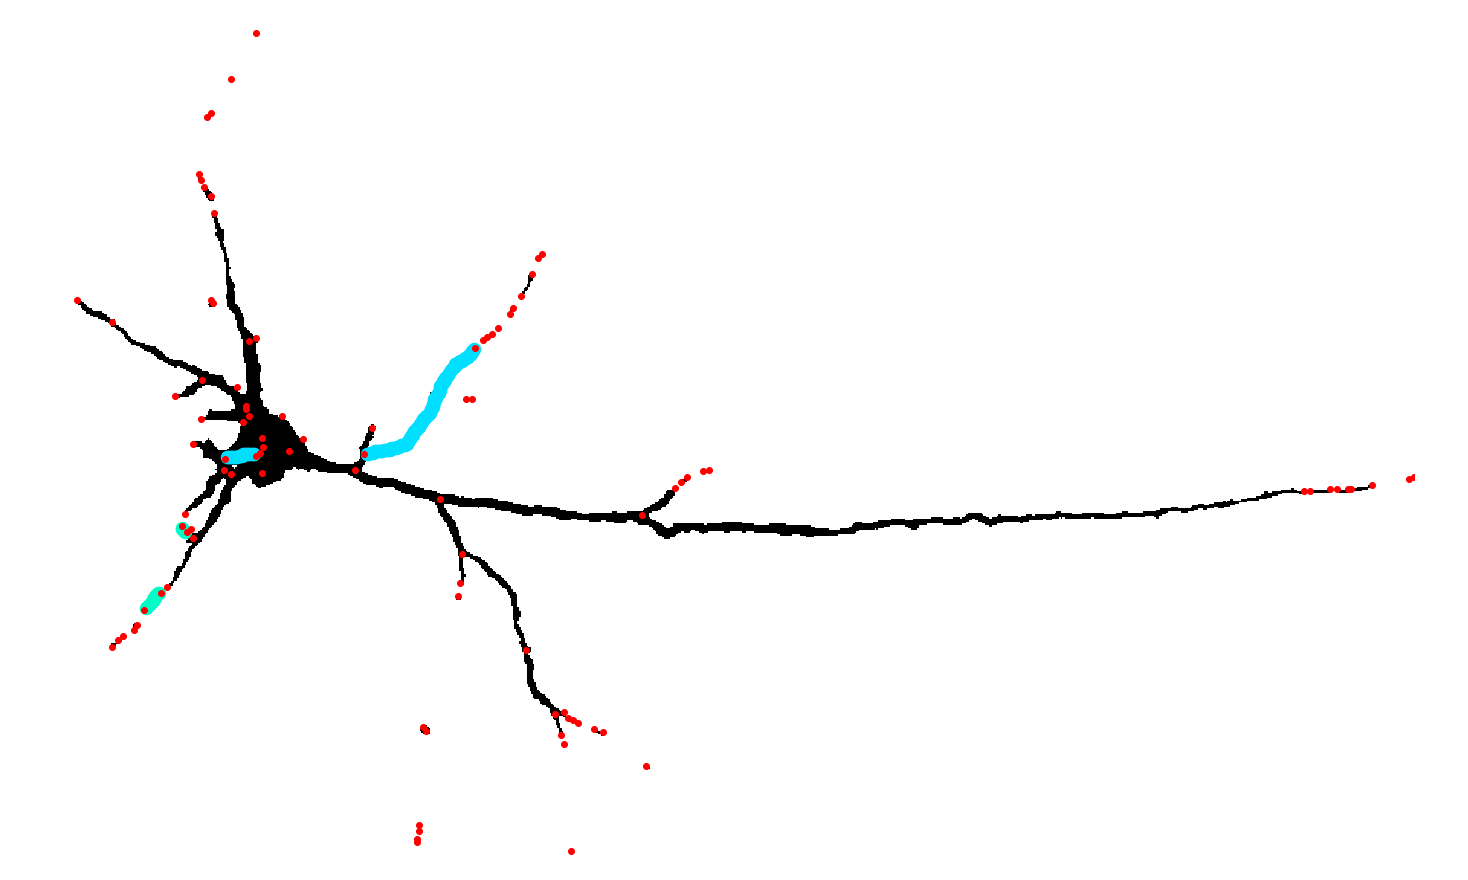
\includegraphics[height=1.3in]{Pictures/Porta18-3a1-phil-s10-v056-exactMatch-antLabeled.png}
                \caption{Muestra N3 Calce Exacto}
            \end{figure}
        \end{column}
        \begin{column}{0.45\textwidth}
            \begin{figure}
                \centering
                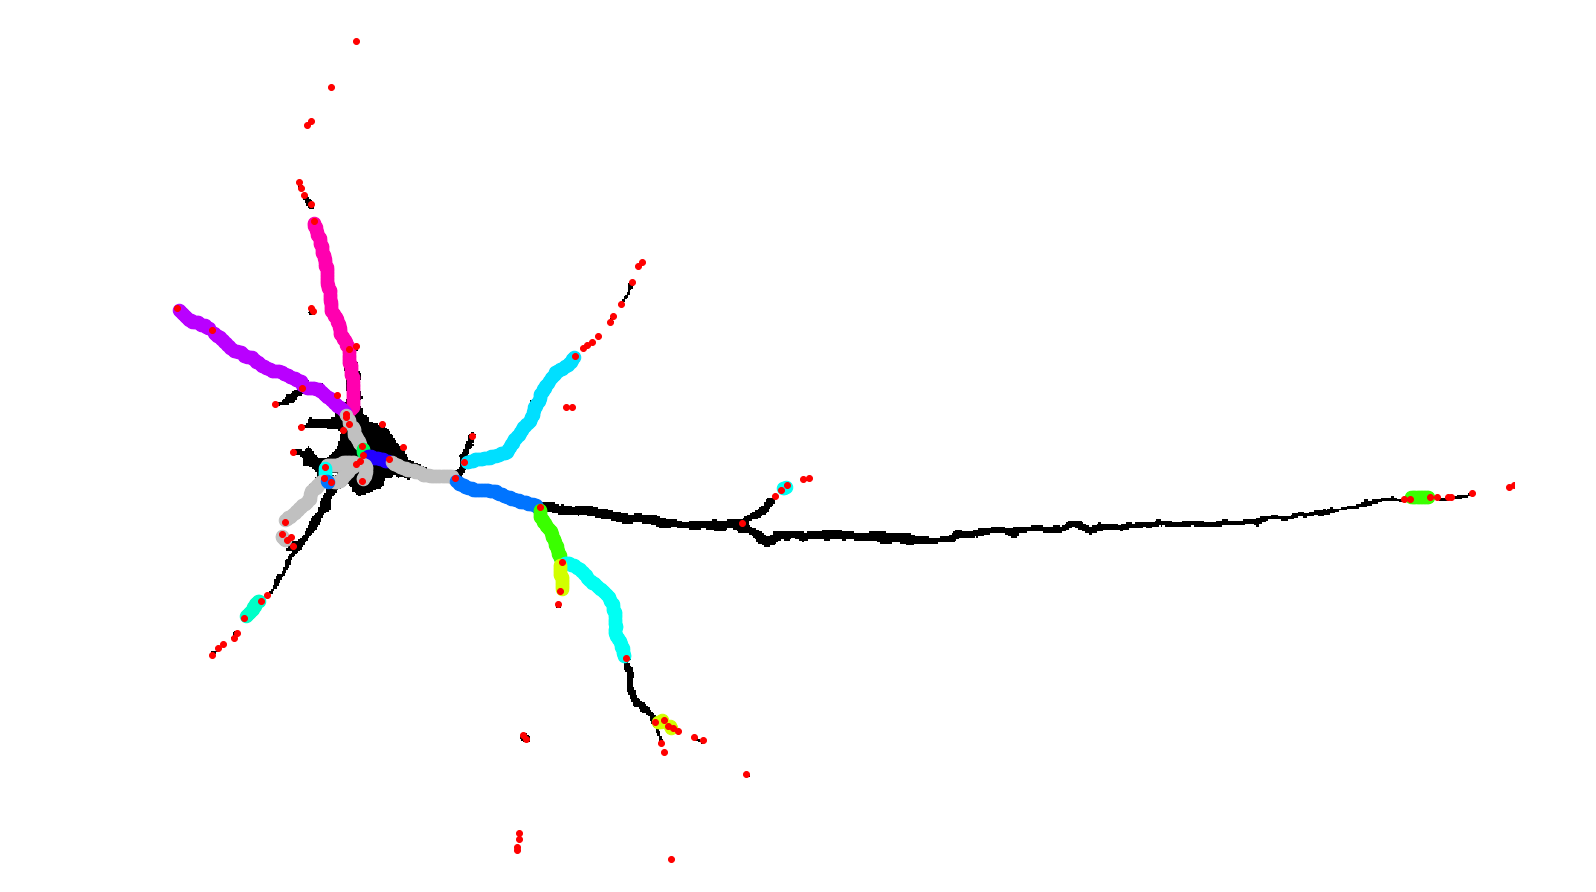
\includegraphics[height=1.3in]{Pictures/Porta18-3a1-phil-s10-v056-overmatches-3-antLabeled.png}
                \caption{Muestra N3 con sub/sobre asignaci\'on}
            \end{figure}
        \end{column}
    \end{columns}
    
    \begin{table}[h]
    \resizebox{\textwidth}{!}{
        \begin{tabular}{|c|c|c|c|c|c|c|c|c|c|c|c|c|}
        \hline
              Muestra & P & P* & R & R* & F1 & F1* & C/P & C/P* & C/GT & C/GT* & F.S. & F.S.* \\ \hline
            N1 & 0.62 & 0.6 & 0.15 & 0.13 & 0.24 & 0.22 & 1.6/59 & 3/66 & 1.6/24 & 3/24 & 1.4 & 1\\
            N2 & 0.2 & 0.21 & 0.09 & 0.1 & 0.13 & 0.14 & 4.6/34.8 & 6/34 & 4.6/29 & 6/29 & {\bf 8} & 7 \\
            N3 & 0.5 & 0.47 & 0.32 & 0.29 & 0.39 & 0.36 & 2/17.4 & 2/17 & 2/14 & 2/14 & {\bf 7.8} & 8\\
            \hline
        \end{tabular}
        }
        \caption{(*) indica el mejor resultado de las 5 iteraciones}
    \end{table}
\end{frame}

\note[itemize]{
  \item a\'un cuando los calces exactos son bajos, existen varios filamentos propuestos que se encuentran en un rango de 1 a 3 aristas faltantes o sobrantes, con respecto a un filamento correcto.
  
  \item la columna C/P refleja el n\'umero de filamentos correctos con respecto a los propuestos por cada m\'etodo, mientras que la columna C/GT indica la relaci\'on entre los filamentos correctamente individualizados por el m\'etodo y el criterio del experto. Finalmente la La columna F.S. indica el n\'umero de filamentos cuya diferencia con respecto a ser un calce exacto es a lo m\'as de 3 aristas. (*) Las columnas con asterisco representan el m\'aximo obtenido tras las 10 ejecuciones del algoritmo propuesto, mientras que las sin asterisco representan el promedio.
  
  \item Nuevamente el algoritmo presenta un comportamiento balanceado en sus 10 iteraciones, donde el mejor resultado no se diferencia demasiado del promedio.
}

\begin{frame}{Resultados Generales (OE 4)}
\resizebox{\textwidth}{3.1cm}{
    \begin{tabular}{|c|c|c|c|c|}
        \hline
        Figura & Config. & Fil. Correctos & Fil. Propuestos & $p$-value  \\ \hline
         4.1 & S1  & 6 & 5.9 & {\bf 1} \\
         4.2 & S2 & 5 & 8.5 & 0.003\\
         4.3 & MtP & 12 & 12.4 & {\bf 0.125}\\
         4.4 & MtP & 12 & 15 & 0\\
         4.5 & MtP & 5 & 5 & {\bf 1}\\
         4.6 & N & 24 & 60.2 & 0\\
         4.7 & N & 29 & 34.3 & 0\\
         4.8 & N & 14 & 17.6 & 0.003\\ 
         5.3b & MtP & 19 & 21 & 0.001\\
         5.3c & MtP & 23 & 29.4 & 0 \\
         5.9a & MtP & 13 & 14 & 0.001\\
         5.10a & MtP & 12 & 13.1 & 0\\
         \hline
    \end{tabular}
}
\end{frame}

\note[itemize]{
    
    \item El hecho que el algoritmo propuesto no tenga diferencias estadísticamente significativas en 3 de las pruebas, as\'i como que presente un n\'umero de filamentos propuestos cercano a lo indicado por un experto en la mayor\'ia de los casos representa la capacidad del algoritmo de acotar el espacio de b\'usqueda de forma eficiente
    
    \item Es relevante destacar que la configuraci\'on predefinida para neuronas o para microt\'ubulos de planta no ha sido ajustada o sintonizada. Es probable que con una sintonización de par\'ametros, los resultados mejoren.
    
    \item SKIP Se defini\'o que La hip\'otesis nula (H0) fuese la no existencia de diferencia estad\'isticamente significativa entre el n\'umero de filamentos individualizados por el algoritmo propuesto y lo definido por el experto que realiz\'o la individualizaci\'on manual respectiva. En el caso de que el valor $p$ o {\it p-value} sea menor al 5\%, se rechaza H0. 
}


\section{Conclusiones}
\begin{frame}{Conclusiones}
    %cumplimiento de objetivos
% a partir de un grafo con pesos que representa una red de filamentos, cumpliendo con lo indicado como primer objetivo espec\'ifico. En cuanto al cumplimiento de los dem\'as objetivos espec\'ificos, se tiene:
\begin{itemize}
    \item El algoritmo propuesto permite resolver un modelo de optimizaci\'on para individualizar filamentos

    \item Se gener\'o una implementaci\'on que resuelve el modelo de optimizaci\'on presentado, considerando casos de solapamiento y/o cruce
    
    \item Se incorporan diversas caracter\'isticas en el algoritmo propuesto
    %\item  {\bf Identificar la ponderaci\'on de propiedades que entregue mejores resultados para grafos que representen una neurona, una bacteria y una c\'elula eucariota de planta:}: Se realiza una ponderaci\'on de las propiedades utilizadas en el algoritmo propuesto en la secci\'on ..., la que var\'ia dependiendo del tipo de c\'elula y se encuentra asociado a la distribuci\'on de las caracter\'isticas en las distintas etapas de la metaheur\'istica ACO.
    
    \item Se eval\'ua el algoritmo propuesto con respecto a DeFiNe
  %  \item {\bf Evaluar t\'ecnicas que usan s\'olo herramientas de visi\'on por computador, basadas en poblaci\'on de p\'ixeles y otras que utiliza un m\'etodo derivado de contornos activos:} Las t\'ecnicas indicadas se encuentran descritas en el cap\'itulo..., y se enfocan en la extracci\'on de informaci\'on geom\'etrica y/o topol\'ogica. Sin embargo no realizan individualizaci\'on de filamentos, por lo que la evaluaci\'on fue dirigida hacia la investigaci\'on que da lugar a DeFiNe, que si realiza este procedimiento, siendo evaluada en el cap\'itulo ...
  \item Se obtiene un comportamiento estable del algoritmo propuesto
  %\item La flexibilidad del algoritmo propuesto permite 
\end{itemize}
\end{frame}

% \begin{frame}{Conclusiones}
%     \item Como cotinuaci\'on de esta investigaci\'on se encuentra la opci\'on de intensificar la extracci\'on de informaci\'on topol\'ogica y espacial que permita realizar la asociaci\'on de secciones importantes de los filamentos o elementos alrededor de estos en la c\'elula observada, con el fin de seguir a\~nadiendo informaci\'on al modelo. Tambi\'en es posible vislumbrar una extensi\'on de este trabajo en la identificaci\'on de las interacciones entre los filamentos individualizados. Lo anterior se refleja en microt\'ubulos como la identificaci\'on de interacciones tipo cat\'astrofe, zippering o nucleaci\'on, mientras que para una neurona ser\'ia la clasificaci\'on autom\'atica de los filamentos en axon o dendritas primarias o secundarias.
% \end{frame}
% TITLE PAGE	

{
\setbeamertemplate{headline}{} %define local, empty header for title page
\setbeamertemplate{footline}{} %define local, empty footer for title page
\maketitle
}
\addtocounter{framenumber}{-1} % We don't count the title page

\addtocontents{toc}{\protect\setcounter{tocdepth}{0}}
\section{Anexo}

\begin{frame}{Heur\'istica Miope}
    \begin{equation}%\fontsize{9pt}{7.2}\selectfont
    \eta_{ij} = 
        \begin{cases} 
        \text{Max\_Score si } \measuredangle(c_{ij}, s_{n}^{P}) \in [0, \theta],\\[3ex]
        
        \text{Max\_Score} \cdot \left(1 - \dfrac{ \left| \measuredangle(c_{ij}, s_{n}^{P}) - \frac{\theta}{2} \right|} {180} \right)  \text{ si } \measuredangle(c_{ij}, s_{n}^{P}) \in \quad ]\theta, \text{Max\_Angle}],\\[3ex]
        
        \text{0 en otro caso.}
        \end{cases}
    \end{equation}    
\end{frame}

\begin{frame}{VI, \'Indice Rand e \'Indice Jaccard}
\resizebox{\textwidth}{!}{
    \begin{tabular}{|c|c|c|c|c|c|}
        \hline
        Figura & Config. de Par\'ametros & VI Max & VI & Rand & Jaccard \\ \hline
         4.1 & MT-P  & 2.3978 & 1.6360 & 0.7646 & 0.2485 \\
         4.1 & S1  & 2.3978 & 0.7091 & 0.8637 & 0.4750  \\
         4.2 & MT-P & 3.0445 & 2.2296 & 0.7276 & 0.1806 \\
         4.2 & S2 & 3.0445 & 2.5878 & 0.7276 & 0.1673  \\
         4.3 & MT-P & 3.4965 & 2.1656 & 0.8658 & 0.2407 \\
         4.4 & MT-P & 3.7612 & 2.6285 & 0.8683 & 0.2488  \\
         4.5 & MT-P & 1.9459 & 0.4286 & 0.8929 & 0.40 \\
         4.6 & N & 6.0258 & 1.7950 & 0.8864 & 0.1389 \\
         4.7 & N & 5.0814 & 3.7256 & 0.8775 & 0.0703 \\
         4.8 & N & 4.2046 & 1.0060 & 0.8794 & 0.2157 \\ \hline
    \end{tabular}
    %\caption{VI $\in [0, VI\_Max]$, Rand y Jaccard $\in [0, 1]$ }
}
\end{frame}

\begin{frame}{VI, \'Indice Rand e \'Indice Jaccard}
%    La mayor\'ia de los criterios para comparar particiones mediante conteo de pares   se basa en la 
    
    %suele fundamentarse en el uso de la matriz de confusi\'on, tambi\'en llamada matriz de asociaci\'on o tabla de contingencia \cite{meilua2007comparing}. Esta tabla considera 4 casos en los que puede estar un par de elementos del {\it data set}, que para el caso de la individualizaci\'on de filamentos son pares de aristas, en las particiones $C$ y $C'$:

    \begin{itemize}\fontsize{9pt}{10}\selectfont
        \item Mayor\'ia de los criterios para comparar particiones $\rightarrow$ matriz de confusi\'on/asociaci\'on o tabla de contingencia.
        \item $N_{11}$: N\'umero de pares que est\'an en el mismo cluster en $C$ y $C'$
        \item $N_{00}$: N\'umero de pares que est\'an en distintos clusters en $C$ y $C'$
        \item $N_{10}$: N\'umero de pares que est\'an en el mismo cluster en $C$ pero no en $C'$
        \item $N_{01}$: N\'umero de pares que est\'an en el mismo cluster en $C'$ pero no en $C$
        \item $N_{11} + N_{00} + N_{10} + N_{01} = \frac{n(n-1)}{2}$, con n como el n\'umero de aristas.
        \item Asociaci\'on de casos con evaluaciones de clasificaci\'on
    \end{itemize}

    %\resizebox{\textwidth}{!}{
    \makebox[\linewidth][c]{\fontsize{10pt}{12}\selectfont
        \begin{tabular}{|c|c|}
        \hline
            Casos para un par de aristas & Clasificaci\'on \\ \hline
            $N_{11}$ & Verdadero Positivo ({\it True Positive} o TP) \\
            $N_{00}$ & Verdadero Negativo ({\it True Negative} o TN)\\
            $N_{10}$ & Falso Positivo ({\it False Positive} o FP)\\
            $N_{01}$ & Falso Negativo ({\it False Negative} o FN)\\ \hline
        \end{tabular}
    }
\end{frame}

\begin{frame}{\'Indice Rand y Jaccard}
    \begin{equation}\fontsize{9pt}{7.2}\selectfont
        \mathcal{R}(C,C^{\prime}) = \frac{N_{11} + N_{00}}{n(n-1)/2} = \frac{TP + TN}{TP + TN + FP + FN}
    \end{equation}
    \vspace{0.2cm}
    \begin{equation}\fontsize{9pt}{7.2}\selectfont
        \mathcal{J}(C,C^{\prime}) = \frac{N_{11}}{N_{11} + N_{01} + N_{10}} = \frac{TP}{TP + FP + FN}
    \end{equation}
    \vspace{0.2cm}
    \begin{equation}\fontsize{9pt}{7.2}\selectfont
        \text{Precision} = \frac{TP}{TP + FP}
    \end{equation}
    \vspace{0.2cm}
    \begin{equation}\fontsize{9pt}{7.2}\selectfont
        \text{Recall} = \frac{TP}{TP + FN}
    \end{equation}
\end{frame}


\begin{frame}{Curvatura de una soluci\'on y Magnitud de desplazamiento entre segmentos}
    \centering
    \begin{equation}\fontsize{9pt}{7.2}\selectfont
    \tau_{ij} \leftarrow
        \begin{cases}
        \tau_{ij} \cdot \gamma \text{ si } \measuredangle(proy(\Vec{p}), \Vec{q}) \geq \theta \cdot \text{Max\_Axial\_Displacement},\\[3ex]
        
        \text{0 si } \tau_{ij} \leq 0.25, \\[3ex]
        \tau_{ij} \quad \text{en otro caso.}
        \end{cases}
    \end{equation}
    \vspace{1cm}
    \begin{equation}\fontsize{9pt}{7.2}\selectfont
    \tau_{ij} \leftarrow
        \begin{cases}
        \begin{split}
         \tau_{ij} \cdot \gamma \text{ si } & \sin(\measuredangle seg^{a}_{pMaxMin}) > seg^{a}_{iMax} \cdot 0.1 \cdot \text{Max\_Axial\_Displacement} \\ & \land \measuredangle seg^{a}_{pMaxMin}) > \theta,
        \end{split}
        \\[3ex]
        
        \text{0 si } \tau_{ij} \leq 0.25, \\[3ex]
        \tau_{ij} \quad \text{en otro caso}.
        \end{cases}
\end{equation}
\end{frame}

% \begin{frame}{Ponderaci\'on de las caracter\'isticas}
%     \begin{itemize}\fontsize{9pt}{12}\selectfont
%     \item No es posible utilizar un \'unico par\'ametro para obtener una ponderaci\'on directa
%     %El uso de diversas caracter\'isticas en distintas partes del algoritmo propuesto
    
%     %Dado que las diversas caracter\'isticas utilizadas en el algoritmo propuesto se encuentran en distintos m\'etodos de la metaheur\'istica ACO, 
%     \item Construcci\'on de soluciones: $\frac{100}{n}$\% el grado de los nodos, y el remanente para el \'angulo entre aristas, con $n$ como el n\'umero de aristas.
%     \item M\'etodo de b\'usqueda no local: 100\% posici\'on de la arista.
%     \item Actualizaci\'on de feromonas: 50\% curvatura, 50\% diferencia de magnitud entre segmentos. En el caso espec\'ifico de las neuronas, corresponde a $33.\overline{3}\%$ curvatura, $33.\overline{3}\%$ diferencia de magnitud entre segmentos y $33.\overline{3}\%$ informaci\'on topol\'ogica de centralidad.
% \end{itemize}
% \end{frame}

\end{document}